	\documentclass[a4paper,11pt,dvipsnames]{article}
	\usepackage[english]{babel}
	\usepackage{soul}
	\usepackage{microtype}
	\usepackage{mathtools}
	\usepackage{amssymb,amsmath,amsfonts}
	\usepackage[utf8]{inputenc}
	\usepackage{graphicx}
	\usepackage{geometry}
	\usepackage{float}
	\usepackage{csquotes}
	\PassOptionsToPackage{hyphens}{url}\usepackage{hyperref}
	\usepackage{bigstrut}
	\usepackage{fancyhdr}
	\usepackage{gensymb}
	\usepackage{units}
	\usepackage{booktabs}
	\usepackage{hhline}
	\usepackage[table]{xcolor}
	\usepackage{capt-of}
	\usepackage{multirow}
	\usepackage[export]{adjustbox}
	\usepackage[nottoc,numbib]{tocbibind}
	%\usepackage[super,comma]{natbib}
	\usepackage{titling}
	\usepackage{datetime}
	\usepackage{lipsum}
	\usepackage{wrapfig}
	%\usepackage{subfig}
	\usepackage{subcaption}
	\usepackage{cancel}
	\usepackage{chngpage}
	\usepackage{comment}
	
	\usepackage[
        backend=biber,
        style=alphabetic,
        sorting=ynt
        ]{biblatex} %Imports biblatex package
    \addbibresource{biblio.bib}
    \addbibresource{pedregosa11a.bib}%Import the bibliography file
    
    
	\definecolor{blunipi}{RGB}{43,68,111}
	%\setlength{\columnseprule}{0.1pt}
	\setlength{\columnsep}{20 pt}
\renewcommand{\thefootnote}{\textit{\alph{footnote}}}
	
	\geometry{a4paper, left=20mm, right=20mm, top=30mm, bottom=30mm}
	
	\title{Mining Glasgow Norms} 
	\author{Data Mining I Project}
	\date{\today}
	
	\pagestyle{fancy}
	\lfoot{Data Mining I Project}
	\rfoot{Mining Glasgow Norms} 
	
	\begin{document}

		\newgeometry{left=14mm, right=13.5mm, top=13.5mm, bottom=30mm}
		\begin{titlepage}
			\thispagestyle{empty}
			\begin{figure}
				
\includegraphics[width=31.5mm,right]{./Cherubino}
			\end{figure}
			\vspace*{-35mm}\hspace{-6mm}\textbf{\textcolor{blunipi}{\large{Dipartimento di Informatica}}}\\\\
			\textcolor{blunipi}{\large{Università di Pisa}}
			
			\vspace{30mm}
			\begin{center}
				\textcolor{blunipi}{\huge{\textbf{\thetitle}}}\\\vspace*{10mm}
				\textcolor{blunipi}{\theauthor}\\\vspace*{10mm}
				\textcolor{blunipi}{\thedate}\\\vspace*{20mm}


				\begin{tabular}{ll}
					\textbf{Authors:}
					
					& Giulio Cordova \\
					& 588294 \\
					& \texttt{g.cordova@studenti.unipi.it}\\\\
					
					& Moreno D'Alfonso \\
					& 627885 \\
					& \texttt{m.dalfonso@studenti.unipi.it}\\\\
					
					& Bruno Javier Limon Avila \\
					& 646137 \\
					& \texttt{b.limonavila@studenti.unipi.it}\\\\
					
					& Elena Scaglione \\
					& 645638 \\
					& \texttt{e.scaglione1@studenti.unipi.it}\\\\
					
					


					
				\end{tabular}
			\end{center}
		\end{titlepage}

		\makeatother
		\pagenumbering{Roman} % Start roman numbering
		\restoregeometry
	\onecolumn \tableofcontents
%\twocolumn
		\newpage
		%\setcounter{page}{1} % Set the page counter to 3
\pagenumbering{arabic} % Start roman numbering
\section{Data Understanding \& Preparation}
The \textit{Glasgow Norms} are a set of ratings of English words based on 9 different parameters (\textit{arousal}, \textit{valence}, \textit{dominance}, \textit{concreteness}, \textit{imageability, familiarity, age of acquisition, size, gender}). These parameters will be described during this section of the report, other aspects will be discussed in further sections. Additionally, there are other variables (not in the \textit{Glasgow Norms} set) useful for the analysis, such as the \textit{length} and a \textit{polysemy} index for each word, and the \textit{frequency} of the word found in the Google \textit{web corpus}. The provided dataset consists of 4682 unique words. 


\subsection{Data Semantics}\label{semantic}
In the next paragraphs the variables will be analyzed one by one. 
%dividiamoci le definizioni:




\paragraph{Arousal} (continuous numerical) indicates how much excitement is felt by the person interviewed when reading the word. Its range varies from 1 to 9, where 1 means very calm and 9 very excited. This parameter is an indicator of the emotional impact of the word.
%Its mean is 4.68 and its Standard Deviation is 1.10. All the statistical information can be seen in Table \ref{tab:stat}, and its distribution in Figure \ref{fig:ardis}.
%
\paragraph{Valence} (continuous numerical) is a measure of how much the object is valuable . The range varies from 1 to 9, where 1 is a low value indicator and 9 high value. The meaning of value is not specified in the dataset. It could be interpreted in a sense of economics or also personal (affection, etc.). Like \textit{arousal}, this parameter is also an indicator of the emotional impact of the word.
%Its mean is 5.09 and its Standard Deviation is 1.59. All the statistical information can be seen in Table \ref{tab:stat}, and its distribution in Figure \ref{fig:valdis}.
%
\paragraph{Dominance} (continuous numerical) is the parameter that treats the degree of control that is felt over the object. The range varies from 1 to 9, where 1 is low control and 9 high. This is the last parameter of the emotional impact of the word.
%
%Its mean is 5.04 and its Standard Deviation is 0.93. All the statistical information can be seen in Table \ref{tab:stat}, and its distribution in Figure \ref{fig:domdis}.
%
\paragraph{Concreteness} (continuous numerical) represents the degree to which something can be experienced by our senses. It is a numerical variable that ranges from 1 (more abstract concepts) to 7 (words that refer to people, places and things that can be seen, heard, felt, smelled or tasted).

\paragraph{Imageability} (continuous numerical) measures how difficult is to generate a mental image of something. It is a numerical parameter that ranges from 1, hard to imagine, to 7, easy to imagine. 

\paragraph{Familiarity} (continuous numerical) is a measure of how commonly a word is experienced. The interval scale of this numerical variable is from 1 to 7, based on how familiar participants were with the given word: 1 if they were unfamiliar; 7 if they were greatly familiar. 


\paragraph{Age of Acquisition [aoa]} (continuous numerical) indicates the supposed age in which a person first learned that specific word. Clearly it is not easy to remember at which age a word is learned, and for that reason in this dataset this variables refers to an estimation of the age of acquisition, introducing this parameter. The scale is defined as a series of consecutive 2-year periods from the ages of 0 to 12 years, and a final period referring to 13 years and older. This leads us to define 7 different ranges, 0-2, 2-4, 4-6, 6-8, 8-10, 10-12 and 13+.

%There are 4682 occurrences for this variable. That means that there are no missing values, or NaN. The mean is 4.14, and the standard deviation is 1.25. All the informations about the statistics of the variable are report in Table \ref{tab:stat}

\paragraph{Size} (continuous numerical) is a measure of magnitude expressed in either concrete or abstract terms (big, small). That is, if a word can be associated with adjectives like big or small (e.g. palace or mountain for concrete object, and knowledge or love for abstract ideas). The range adopted varies from 1 to 7, where one is a small object and 7 a big object. 
%The count of occurrences for this variable suggests that there are no missing values. The mean is 4.13 and the standard deviation is just above 1.

\paragraph{Gender} (continuous numerical) refers to how strongly its meaning is associated with male or female behavior. This variable could be very interesting in regards to the social bias that might, or might not, be present. \\
The variable is numerical and has a range that goes from 1 to 7. 
This may make the parameter not self-intuitive. There is no visible correlation between the number and the perceived gender of that word. A speculation is that the higher the value, the more "masculine'' the word is perceived. For example the word \texttt{actor} has a perceived gender value of 5.588, while \texttt{actress} 1.303. This may lead to a transformation of the variable, which will be eventually discussed in another section.
\begin{comment}
\begin{figure}[h]
    \raggedright
    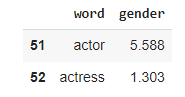
\includegraphics[scale=.9]{Graphs/gender.png}
    \caption{Gender variable}
    \label{figure}
\end{figure}
\end{comment}

\paragraph{Length} (discrete numerical) refers to the size, in number of letters, of each word in the dataset.

\paragraph{Web Corpus Freq} (discrete numerical) is the frequency of any word appearing within the collection of all words contained within the databases of Google Newspapers, which forms a corpus, that is, a body of all words found during a given timeframe and from a specific source. Due to the enormous amount of external factors that might influence the frequency of a word, this variable is the one that shows the biggest variation between results and as such, the most outliers.

\begin{figure*}[ht]
\centering
\begin{minipage}[b]{.3\linewidth}
\centering\large 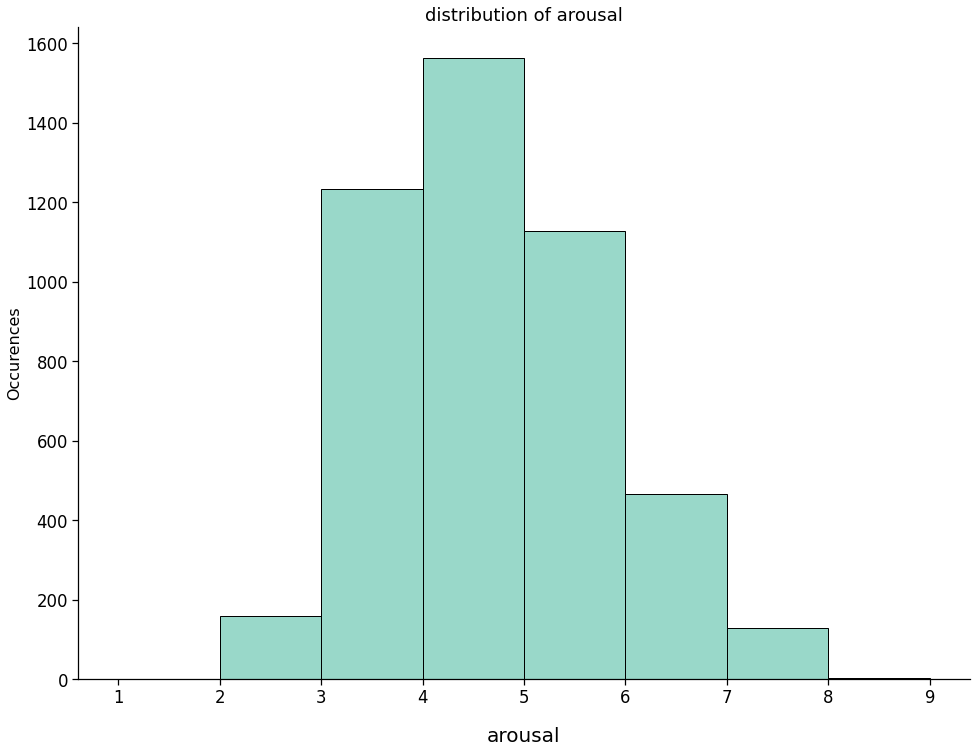
\includegraphics[width=0.9\linewidth]{Graphs/arousal_distributiom.png}
\subcaption{Arousal}\label{fig:ardis}
\end{minipage}%
\begin{minipage}[b]{.3\linewidth}
\centering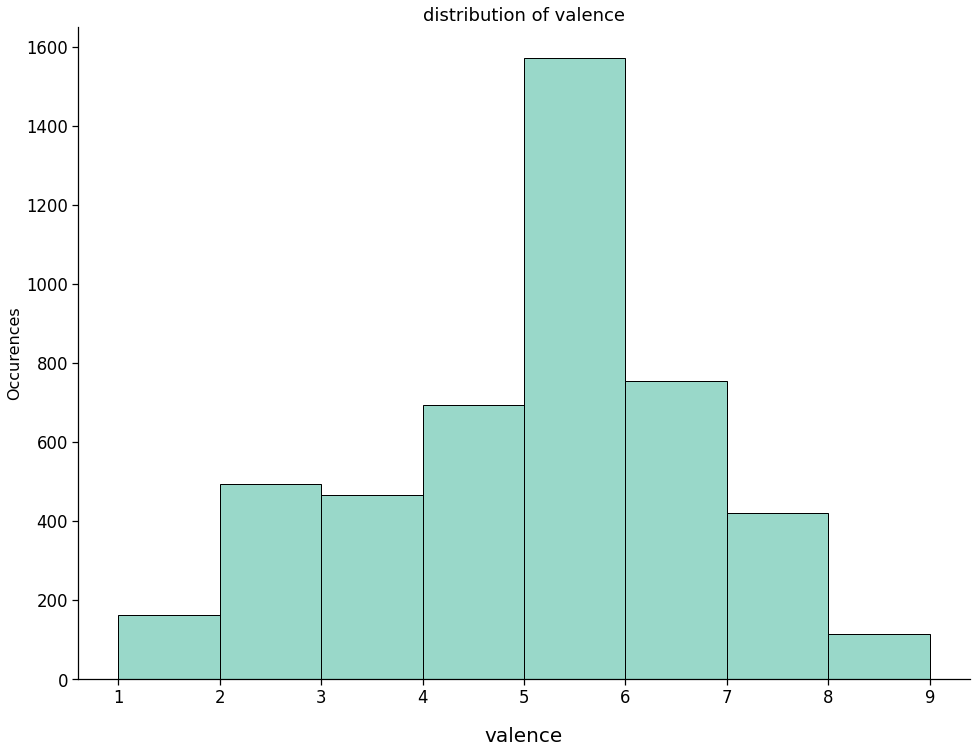
\includegraphics[width=0.9\linewidth]{Graphs/valence_distribution.png}\subcaption{Valence}\label{fig:valdis}
\end{minipage}
\begin{minipage}[b]{.3\linewidth}
\centering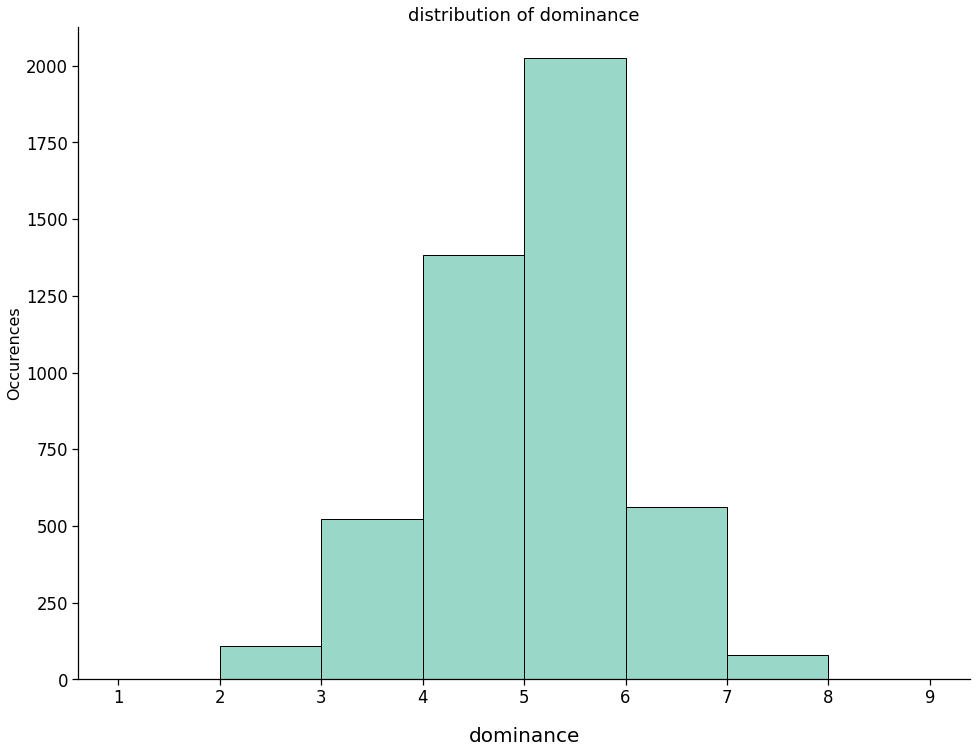
\includegraphics[width=0.9\linewidth]{Graphs/dominance_distribution.png}\subcaption{Dominance}\label{fig:domdis}
\end{minipage}

\begin{minipage}[b]{.3\linewidth}
\centering\large 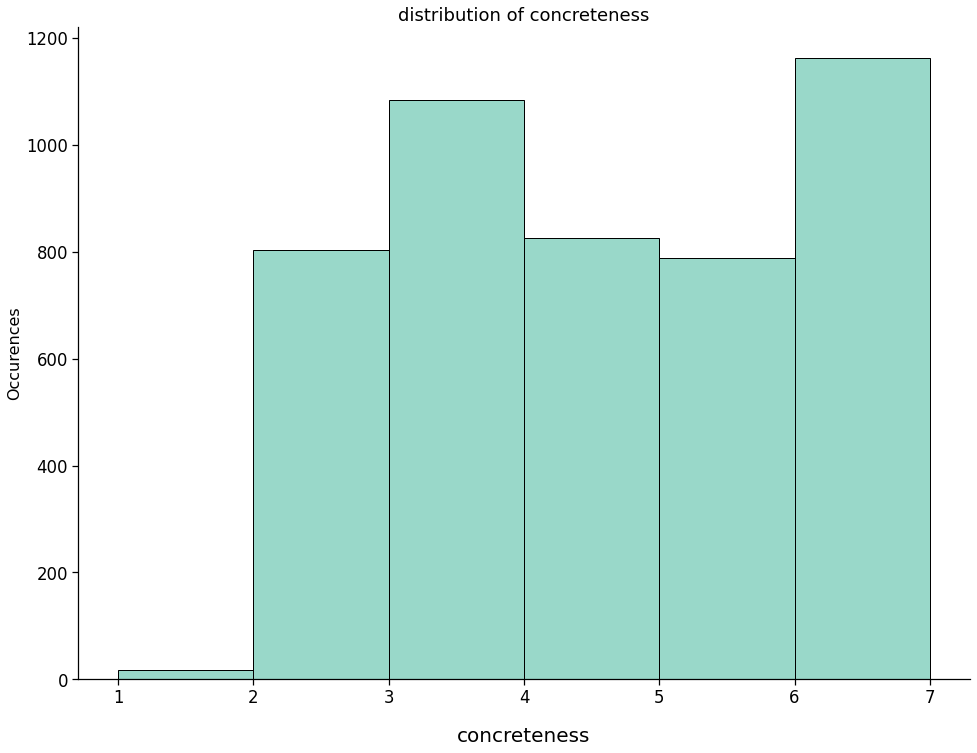
\includegraphics[width=0.9\linewidth]{Graphs/concreteness_distribution.png}
\subcaption{Concreteness}\label{fig:condis}
\end{minipage}%
\begin{minipage}[b]{.3\linewidth}
\centering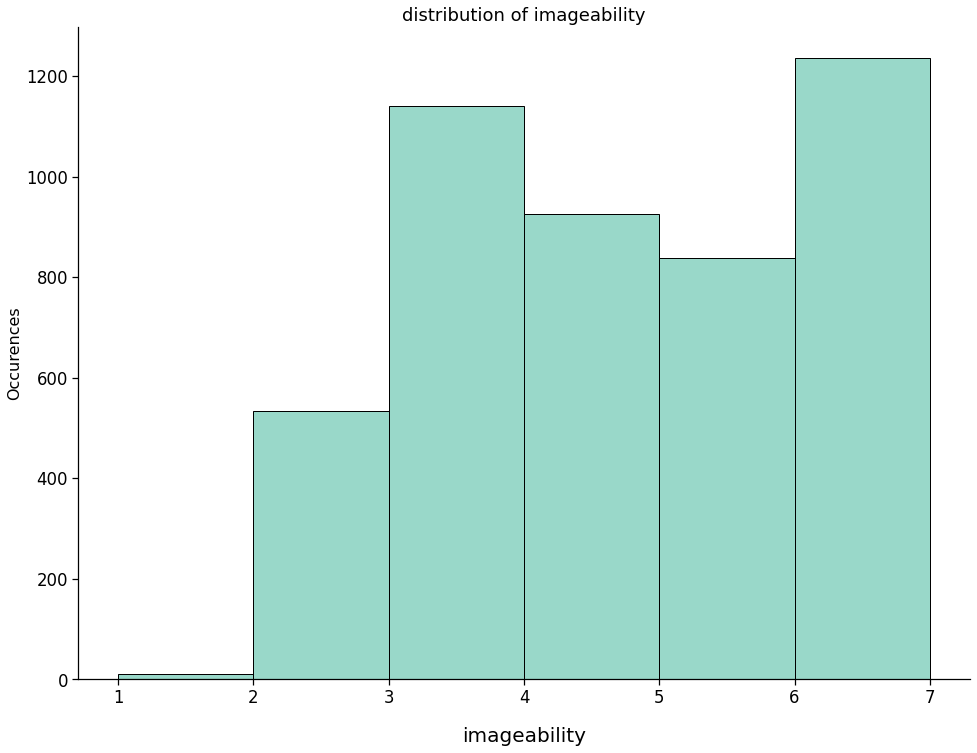
\includegraphics[width=0.9\linewidth]{Graphs/imageability_distribution.png}\subcaption{Imageability}\label{fig:imadis}
\end{minipage}
\begin{minipage}[b]{.3\linewidth}
\centering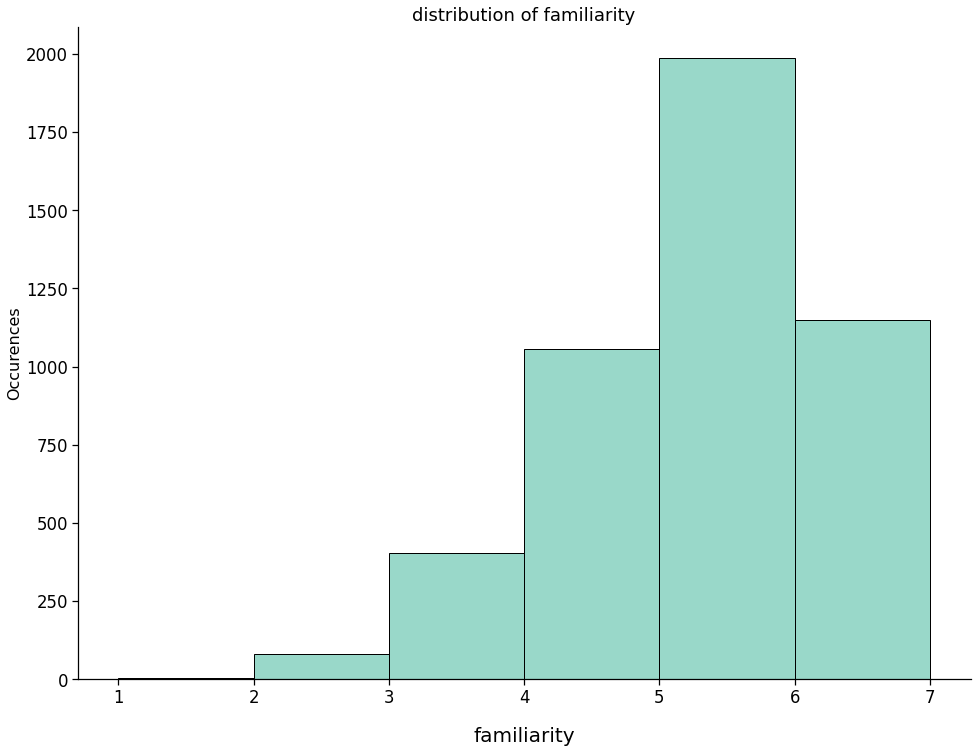
\includegraphics[width=0.9\linewidth]{Graphs/familiarity_distribution.png}\subcaption{Familiarity}\label{fig:famdis}
\end{minipage}

\begin{minipage}[b]{.3\linewidth}
\centering\large 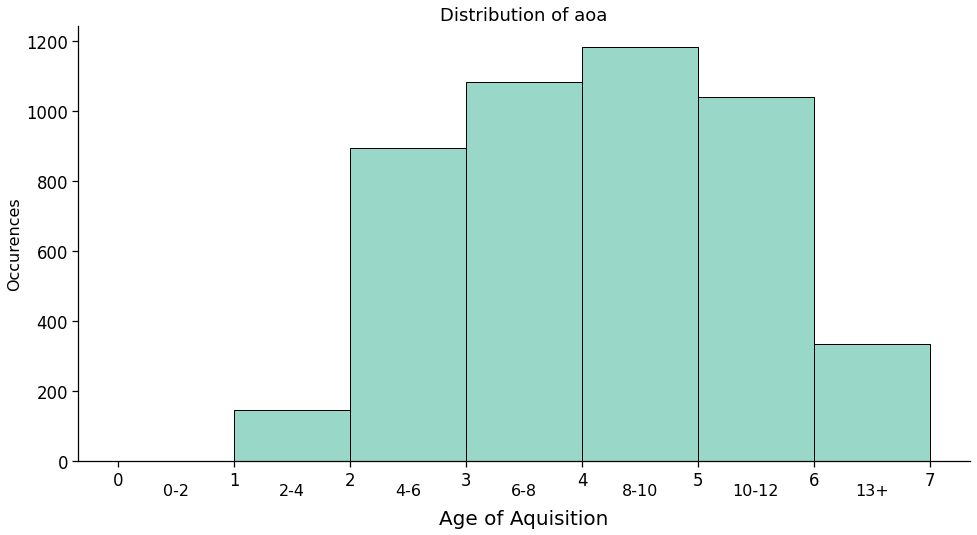
\includegraphics[width=0.9\linewidth]{Graphs/aoa_distribution.png}
\subcaption{Age of Acquisition}\label{fig:aoadis}
\end{minipage}%
\begin{minipage}[b]{.3\linewidth}
\centering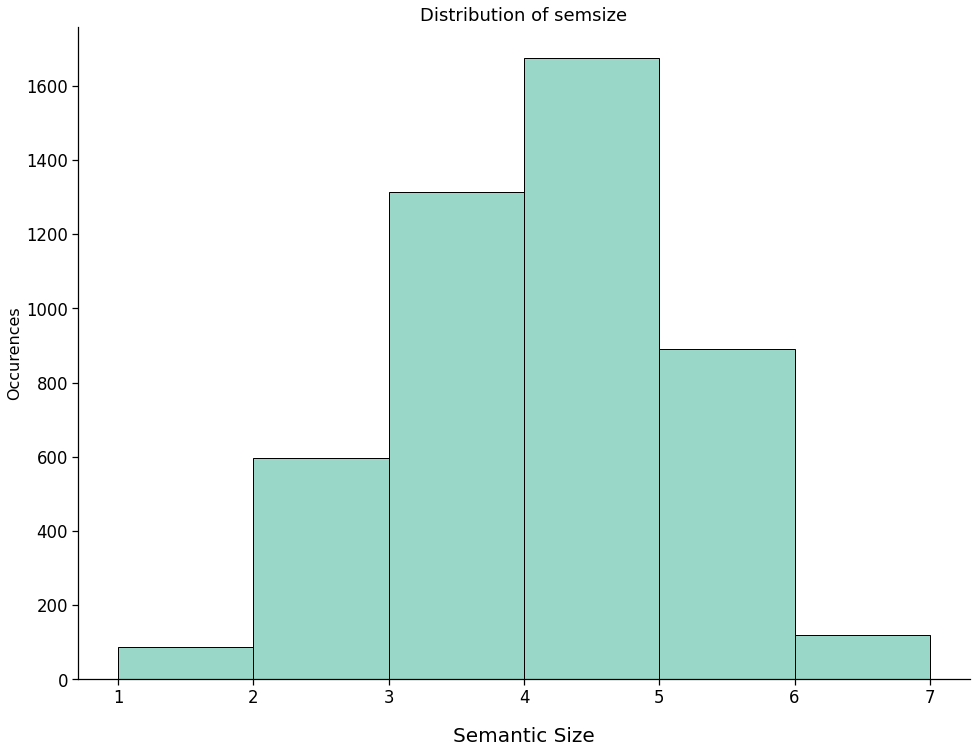
\includegraphics[width=0.9\linewidth]{Graphs/semsize_distribution.png}\subcaption{Size}\label{fig:semdis}
\end{minipage}
\begin{minipage}[b]{.3\linewidth}
\centering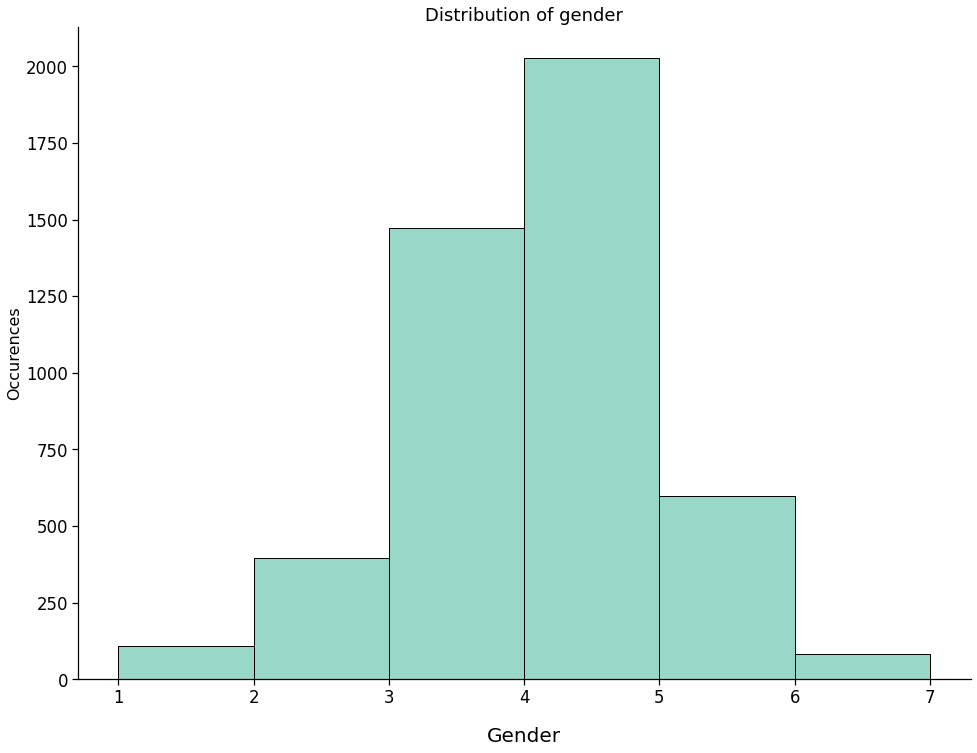
\includegraphics[width=0.9\linewidth]{Graphs/gender_distribution.png}\subcaption{Gender}\label{fig:gendis}
\end{minipage}


\caption{Distributions of variables}\label{fig:dis}

\end{figure*}

\paragraph{Polysemy} (discrete boolean) is a binary variable that denotes the capacity for a word to have multiple related meanings. This relatedness sets it apart from simple homophony, in which the similarity is accidental. Thus, two words with polysemy have a different but related sense, be it historical or etymological, most of the time, this attribution relies on personal judgment.



\subsection[Distributions and statistics]{Distribution of variables and statistics}


A brief overview of the distribution of each variable can be seen in Figure \ref{fig:dis}. 



The parameters \textit{concreteness}, \textit{imageability} and \textit{age of acquisition} tend to a uniform distribution. \textit{Familiarity} is heavily centered on the right side of the graphs, meaning that apparently the words sound very familiar to the readers. It is also the parameter with the smallest standard deviation. \textit{Concreteness} and \textit{imageability} have a distribution similar to a bimodal shape. The other parameters are all middle-centered. To have a better idea of the values, a complete statistical overview of the variables (mean, std deviation, percentile, etc.) is reported in Table \ref{tab:stat}. 

\begin{table}[h]
    \centering
\begin{tabular}{l|r|r|r|r|r|r}    
{} &       Length &      Arousal &      Valence &    Dominance &  Concreteness &  Imageability \\
\hline
count &  4682  &  4682  &  4682  &  4682  &   4682  &   4682  \\
mean  &     6.35 &     4.68 &     5.09 &     5.04 &      4.57 &      4.72 \\
std   &     2.01 &     1.10 &     1.59 &     0.93 &      1.43  &      1.36 \\
min   &     2  &     2.06 &     1.03 &     1.94 &      1.67 &      1.74 \\
25\%   &     5  &     3.85 &     4.12 &     4.53 &      3.24 &      3.52 \\
50\%   &     6  &     4.57 &     5.29 &     5.12 &      4.47 &      4.68 \\
75\%   &     8  &     5.42 &     6.09 &     5.60 &      5.97 &      6.03 \\
max   &    16  &     8.18 &     8.65 &     8.37 &      6.94 &      6.94 \\
range & 1-$\infty$ & 1-9 & 1-9 & 1-9 & 1-7 & 1-7 \\
\hline
%&&&&&&\\
\hline
{} &  Familiarity & Age of Aq &      Size &       Gender &     Polysemy &  Web Cor Freq \\
\hline
count &  4682  &  4682  &  4682  &  4682  &  4682  &     4.67e+03 \\
mean  &     5.27 &     4.14 &     4.14 &     4.10 &     0.08  &     2.98e+07 \\
std   &     0.92  &     1.25  &     1.02  &     0.91  &     0.27  &     8.49e+07 \\
min   &     1.65 &     1.22 &     1.37 &     1  &     0  &     1.28e+04 \\
25\%   &     4.71 &     3.11  &     3.44 &     3.61 &     0  &     1.67e+06 \\
50\%   &     5.44 &     4.18 &     4.19 &     4.12 &     0  &     5.70e+06 \\
75\%   &     5.97 &     5.15 &     4.88 &     4.66 &     0  &     2.23e+07 \\
max   &     6.94 &     6.97 &     6.91 &     6.97 &     1  &     2.02e+09 \\
range & 1-7 & 1-7 & 1-7 & 1-7 & 0/1 & 0-$\infty$ \\
\hline
\end{tabular}
\caption{Basic Statistics of each parameter}\label{tab:stat}

\end{table}
%


%Ci sono variabili da trasfomare? Ad esempio usare scala logaritmica


%MIN, MAX, PERCENTILI

%DISTRIBUZIONE DI OGNI SINGOLA VARIABILE (9 ISTOGRAMMI) CE LE ABBIAMO

%PER I POLISEMI SI PUO' USARE UN PIE CHART

%CALCOLARE UNA MATRICE DI CORRELAZIONE

%VEDERE SE GUARDARE QUALCHE VARIABILE A COPPIA OPPURE NO


\subsection{Assessing Data Quality}
%MORENO
In this section, the quality of the data will be discussed, i.e. missing values, outliers, errors and semantic inconsistencies. This kind of analysis is performed using the pandas library, unless otherwise specified.

\subsubsection{Missing Values}

The dataset seems to be almost free of null values. In fact, there are only 14 NaN, and all are concentrated in the \textit{web\_corpus\_freq} variable, shown in Figure \ref{fig:missing}. Given the small number of missing values, a substitution does not lead to a change in the distribution, so we chose to substitute the 14 NaN with the mean value of \textit{web\_corpus\_freq}.

\begin{figure}[h]
    \centering
    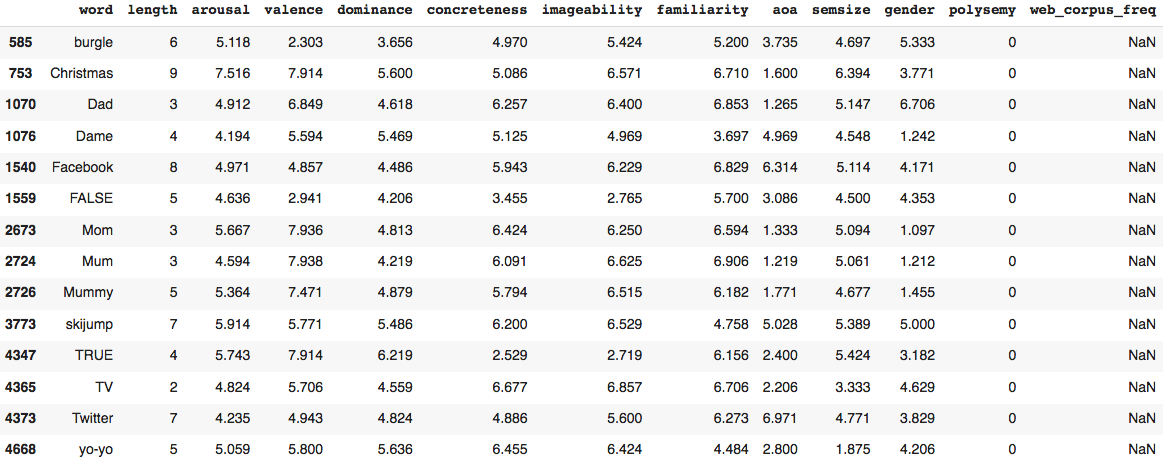
\includegraphics[width=0.8\textwidth]{Graphs/NaN.png}
    \caption{Missing values}
    \label{fig:missing}
\end{figure}
Looking at the values that are present in the dataset but are not present in the web corpus, we can spot some similarities. There are 3 recurrences of the same word but slightly different from one another: \texttt{Mom}, \texttt{Mum} and \texttt{Mommy}. Also the word \texttt{Dad} is not present in the corpus. In addition, there are 3 words written with full capital letters: \texttt{FALSE}, \texttt{TRUE}, and \texttt{TV}. If the corpus is case sensitive, that could be an explanation of why those words are not present.

%MISSING VALUES (NULL, NONE)
%CONTARLI PER COLONNE (E PER RIGHE)
%TOGLIAMO LA COLONNA O LA RIGA? LA RIEMPIAMO? CON CHE VALORE? GUARDIAMO LA DISTRIBUZIONE DELLA VARIABILE 


\begin{figure}[h]
    \centering
    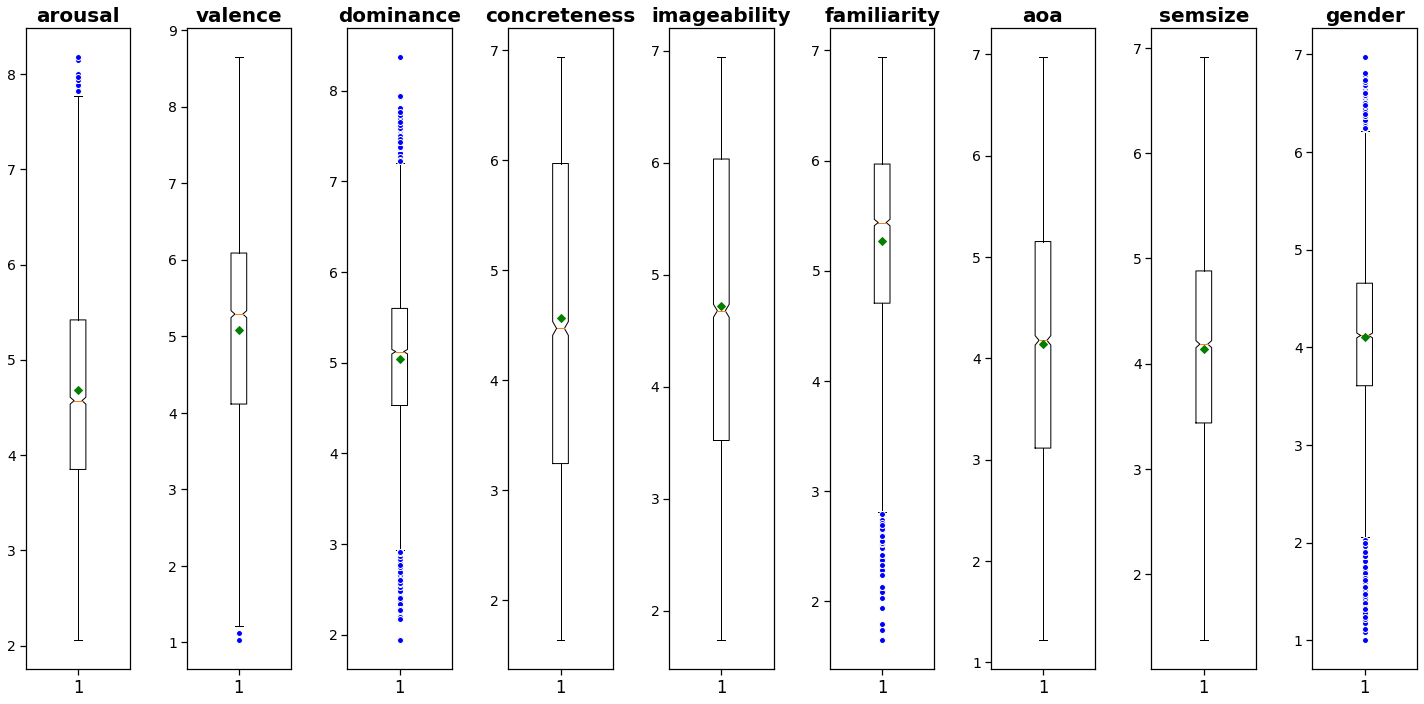
\includegraphics[width=0.7\textwidth]{Graphs/outliers.png}
    \caption{Boxplots for detection of outliers.}
    \label{fig:outliers}
\end{figure}
\subsubsection{Outliers}


First, some variables had to be dropped to perform the boxplot analysis. \textit{word} is not a numerical variable, and for that reason it is not used in this plot. \textit{web\_corpus\_freq} and \textit{polysemy} can be analyzed on their own.


The plot in Figure \ref{fig:outliers} shows that some variables are well distributed, like \textit{concreteness} and \textit{imageability}, while others are not, like \textit{length}, \textit{arousal} and \textit{dominance}. This issue will be later addressed with more depth.

\begin{figure}[h]
\begin{minipage}[b]{.58\linewidth}
    \centering
    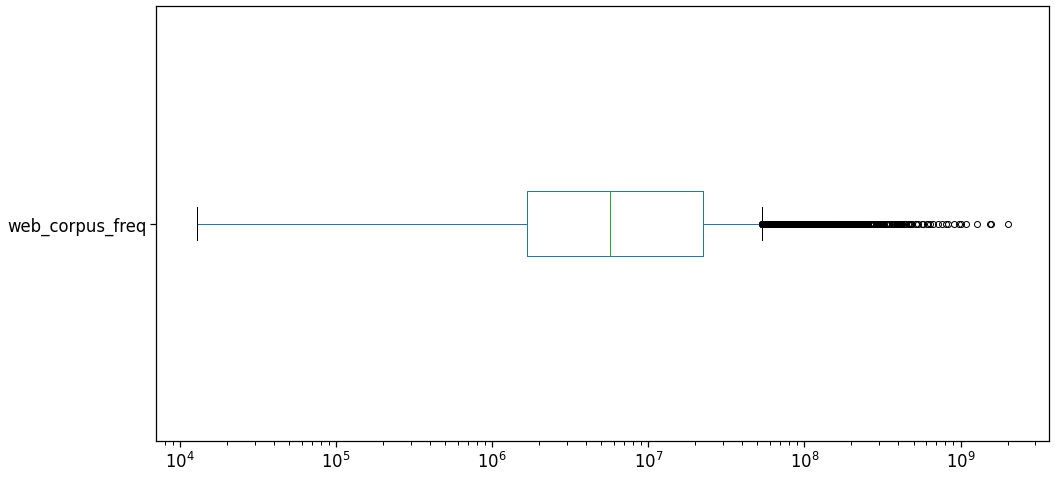
\includegraphics[width=0.7\textwidth]{Graphs/wcf_outliers.png}
    \subcaption{Outliers of the variable \textit{web\_corpus\_freq}. The x axis was transformed using the logarithmic scale.}\label{fig:wcf_outliers}
    \end{minipage}\hfill
    \begin{minipage}[b]{.38\linewidth}
    \centering
    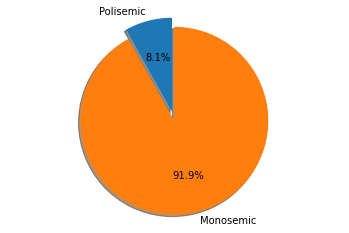
\includegraphics[width=0.7\textwidth]{Graphs/piechart.png}
    \subcaption{Pie Chart of the parameter \textit{polysemy}}\label{fig:pie}
    \end{minipage}
    \caption{Non-standard outliers}
    
\end{figure}

\textit{web\_corpus\_freq} instead seems to have a lot of outliers, as shown in Figure \ref{fig:wcf_outliers}.

\textit{polysemy} has only 2 possible values, 0 and 1, that are \texttt{False} and \texttt{True}. For that reason it does not have outliers. For a better visualization, a Pie Chart is drawn in Figure \ref{fig:pie}.


%OUTLIERS (COME FACCIAMO A VEDERLO?) 
%BOXPLOTS 
%LI TOGLIAMO?

\subsubsection{Errors}
%VARIABILI NUMERICHE VS VARIABILI NON-NUMERICHE, VARIABILI FUORI RANGE, ETC. 
%QUESTI VANNO TOLTI
The errors in this dataset could be some values out of range or values that do not correspond to the datatype. In the Table \ref{tab:stat} one can compare the rows of range and min/max to see that there are no values out of range. With a for loop the datatype of each row was compared to the datatype expected and no errors were found.

Another test was to compare the length of the values of the variable \textit{word} with the values of the variable \textit{length}. The resulting numbers were exactly the same, so there are no errors.


\subsubsection{Semantic Inconsistencies}
%PAROLE CHE SONO INDICATE COME POLISEMICHE MA NON LO SONO, OPPURE IL CONTRARIO
%ALTRE COSE CHE NON CI VENGONO IN MENTE

It is hard to define a semantic inconsistency, given that each word can be interpreted differently by the reader. There are many factors that can influence the understanding of the word such as background, age, origin, education, income, social status etc. Therefore every variable is difficult to evaluate in an unbiased way. 

The one variable that we chose to analyze is polysemy, given its greater objectivity. One can compare all the polysemic word with a definition in a dictionary to check if the word is actually polysemic. Our analysis led to no semantic inconsistencies.

\subsection{Variable transformations}

We did not agree with some choices of the authors for the representation of the variables. In this paragraph it is explained how we decided to transform some variables.

\subsubsection{Gender}

As already said, the variable \textit{gender} is not self intuitive.  An assumption is that  the  higher  the  value,  the  more "masculine'' the word is perceived. For this reason, it was decided to change the name of this variable to \textit{masculinity}.

\subsubsection{Web Corpus Frequency}\label{discretize}

The variable\textit{ Web Corpus Frequency} has a very vast range and does not have an easy comprehension on the linear scale. We decided to discretize the variable with a magnitude to the 10th power that corresponded to that word. For example, if a word occurs $7\cdot10^4$ times in the Google corpus the new value of the variable will be 4; if $web\_corpus\_freq=4\cdot 10^7$ the new value will be 7, and so on. The new range of the variable will be between 4 and 9. 

\subsubsection{Normalization}\label{normalization}

Given that each variable has a different range, it was decided to normalize all the variables between 0 and 1 with the MinMax algorithm, i.e. reshaping the array with new values. The new and transformed variables and normalized as well.

%VEDIAMO SE C'è QUALCOSA DA FARE OPPURE NO, AL LIMITE STA SEZIONE LA TOGLIAMO


\subsection[Pairwise correlations]{Pairwise correlations and elimination of variables}
%FATTA MATRICE  
An overview of the relation between the nine variables is provided in Figure \ref{fig:correlation}. Where a correlation greater than \textbar{0.6}\textbar{} is found, we plotted the values of the two variables for a better visualization (Figure \ref{fig:pairplot}). 

There is a strong correlation that can be seen in Figure \ref{fig:pairplot_ima_conc} between \textit{concreteness} and \textit{imageability}: it is difficult to imagine an abstract word and easier to imagine a concrete one.  Moreover, \textit{concreteness} and \textit{imageability} relate to the other variables similarly, with a margin of \textpm 0.14. Therefore we merged them into a new variable, \textit{perceivability}. The values of \textit{perceivability} are the mean of concreteness and \textit{imageability} values. 

Other positively correlated variables are \textit{valence} and \textit{dominance}, with 0.72: the more valuable an item is perceived, the higher the degree of control over the object, as seen in Figure \ref{fig:pairplot_dom_val}. 
\textit{Familiarity} and \textit{age of acquisition} are instead negatively related: from the pairplot in Figure \ref{fig:pairplot_aoa_fam} is apparent that every word acquired in early age is highly familiar. 


\begin{figure}[h]
    \centering
    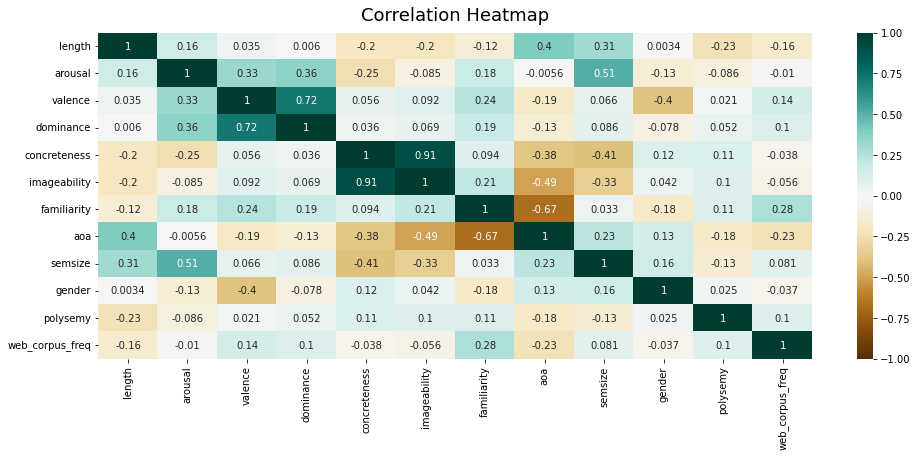
\includegraphics[width=0.8\textwidth]{Graphs/heatmap.png}
    \caption{Pearson Correlation Heatmap of the variables.}
    \label{fig:correlation}
\end{figure}

\begin{figure}[ht]
    \centering
    \begin{minipage}{0.3\textwidth}
    \centering
    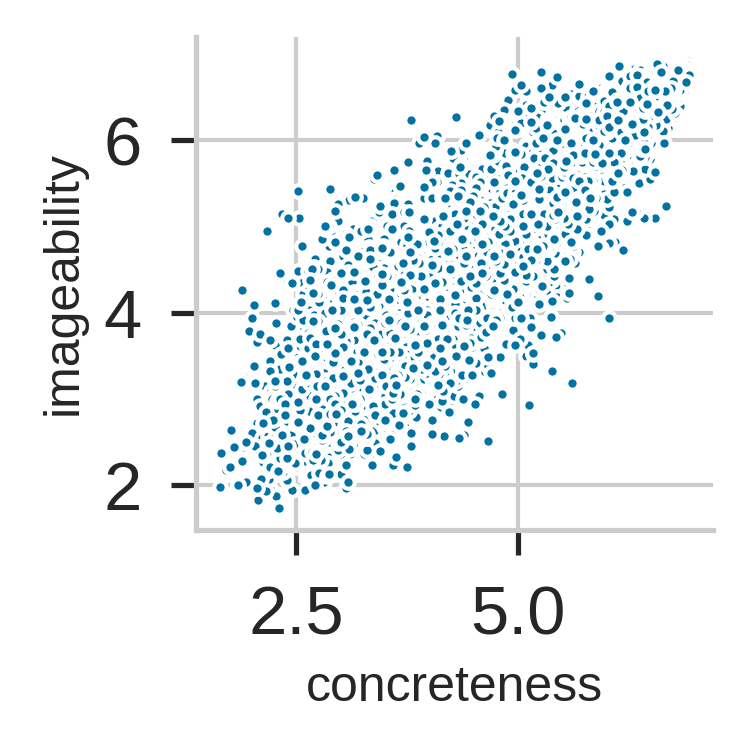
\includegraphics[width=0.65\columnwidth]{Graphs/pp_imageability_concreteness.png}
    \subcaption{Imageability vs Concreteness}\label{fig:pairplot_ima_conc}
\end{minipage}
\begin{minipage}{0.3\textwidth}
\centering
    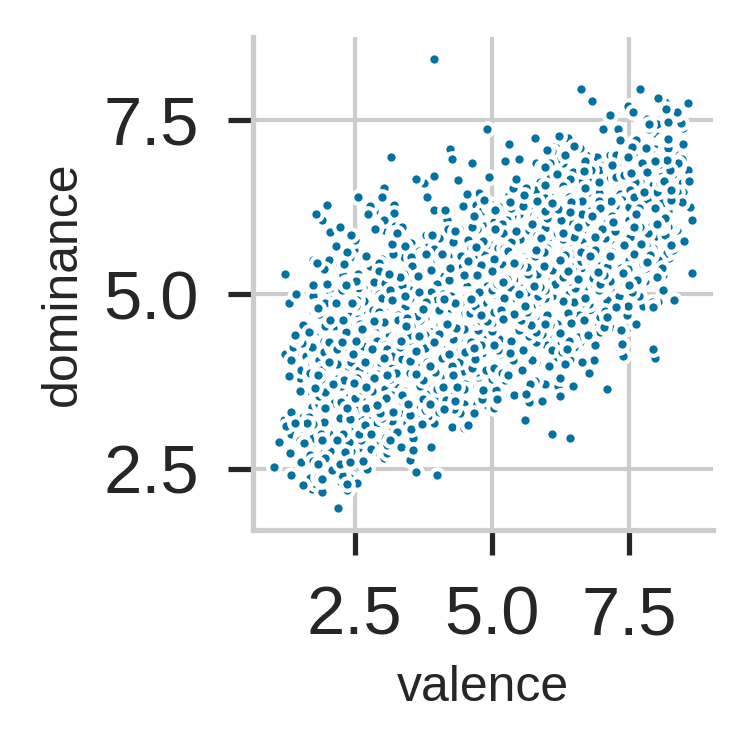
\includegraphics[width=0.65\columnwidth]{Graphs/pp_dominance_valence.png}
    \subcaption{Dominance vs Valence}
    \label{fig:pairplot_dom_val}
    \end{minipage}
    \begin{minipage}{0.3\textwidth}
    \centering
    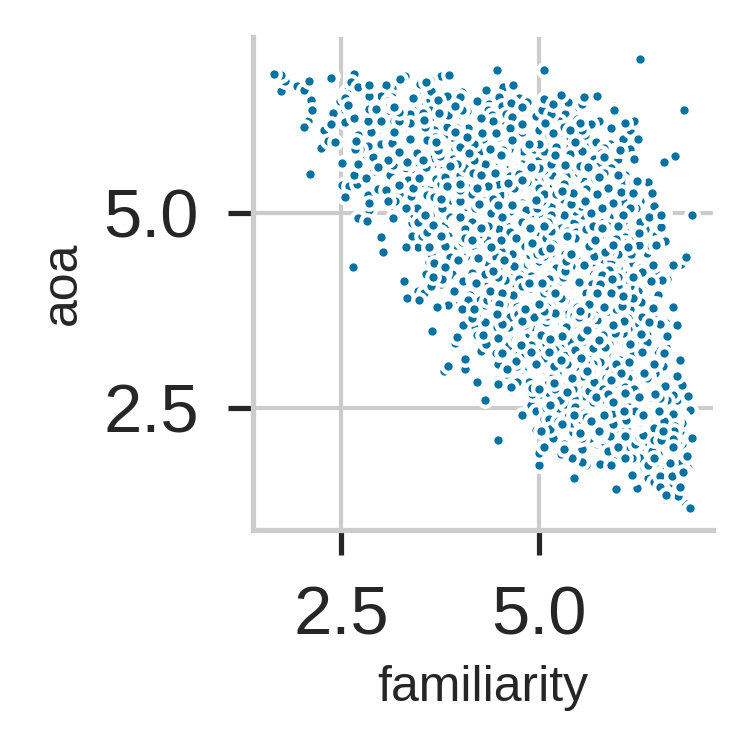
\includegraphics[width=0.65\columnwidth]{Graphs/pp_aoa_familiarity.png}
    \subcaption{Aoa vs familiarity}\label{fig:pairplot_aoa_fam}
        \end{minipage}
        \caption{Pairplot of correlated variables}\label{fig:pairplot}
\end{figure}

\begin{comment}
\begin{figure}
    \centering
    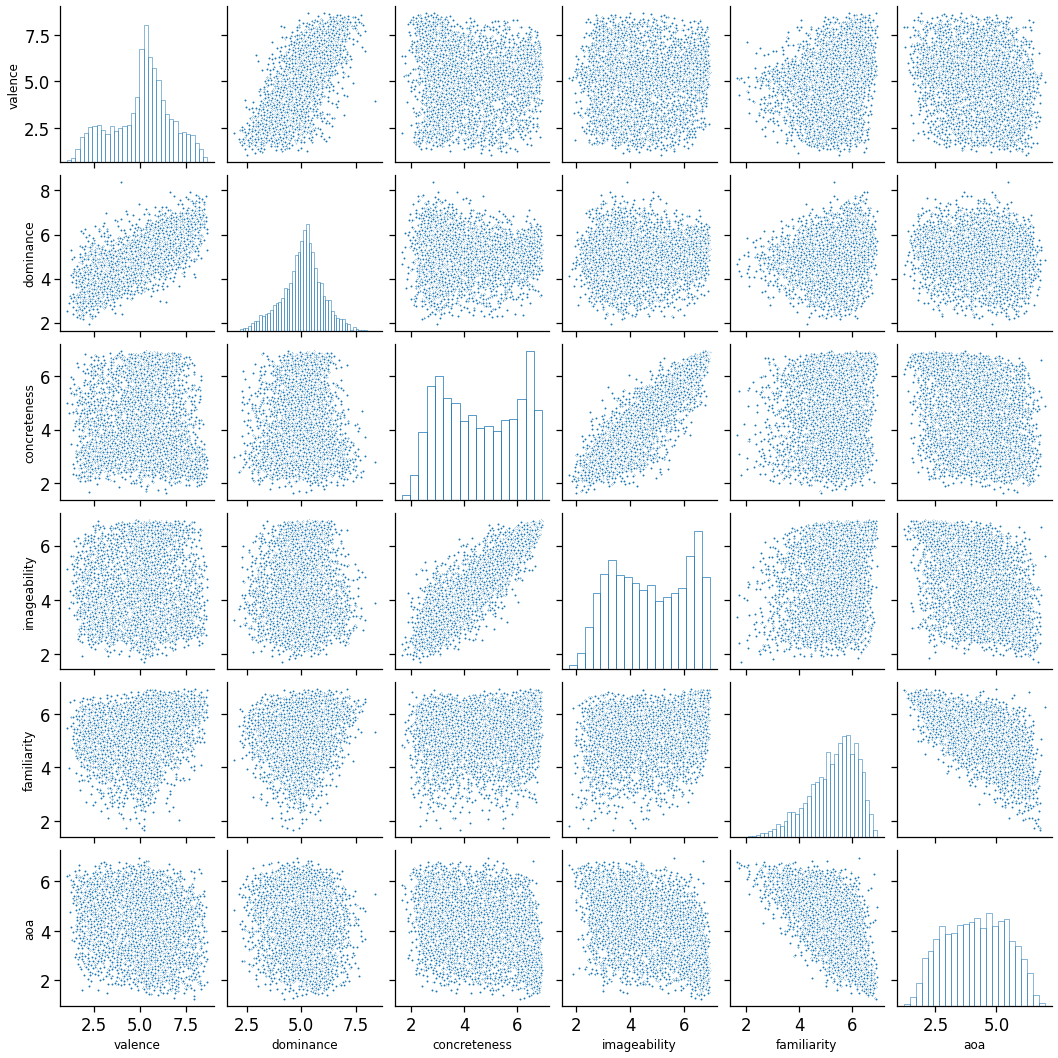
\includegraphics[width=0.8\textwidth]{Graphs/pairplot.png}
    \caption{Pairplot of the variables.}
    \label{fig:pairplot}
\end{figure}
\end{comment}



%Mettiamo i pairplot delle variabili che hanno una correlazione in modulo più alta di 0.6.

%Correlation e Imageabiltiy si correlano ugualmente con tutte le variabili in un intervallo di +-0.14. Quindi si possono unire.

%Ne eliminiamo una e teniamo la media fra le due. La nuova variabile si chiama Perceivability.

%segue dalla matrice di correlazione. Analisi più semplice se ad esempio concretezza familiarità e immaginabilità sono correlate e posso fare una variabile sola 

\subsection{Recap of the preprocessing}

The preprocessing of the dataset is useful not only for a better visualization, but  to have a clean dataset to work with. 


To define it, we will recap what we just did in this section.
First, we made sure that there were no errors or semantic inconsistencies. Then, we substituted the 14 missing values with the average of the missing variable. The variable \textit{gender} was renamed to \textit{masculinity} and the variable \textit{web corpus frequency} was discretized. We unified the variables \textit{concreteness} and \textit{imageability} in a new one, \textit{perceivability}, substituting the mean values of the two original ones. Finally, the whole dataset (except for the variable \textit{word}) was normalized between 0 and 1.
\begin{comment}
The first 5 rows of the dataset we used to perform our analysis are displayed in Figure \ref{fig:ultimate}.

\begin{figure}[h]
    \centering
    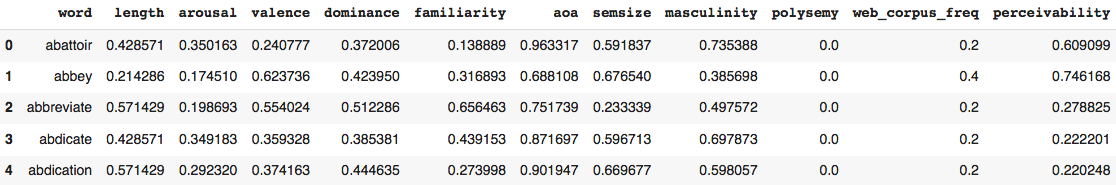
\includegraphics[width=\textwidth]{def.png}
    \caption{First 5 rows of the final dataset to work with}
    \label{fig:ultimate}
\end{figure}
\end{comment}

\section{Clustering}

To evaluate a cluster analysis, three different algorithms are used. Both the algorithms and the obtained results will be described in the following sections.

\subsection{Preprocessing}
As discussed in the previous section, the dataframe has already been reduced and normalized to perform a better analysis. The last thing to do before moving forward is to drop the variable \textit{word}. The statistics of this dataset can be seen in Figure \ref{tab:stat2}.

\begin{figure}[h]
    \centering
    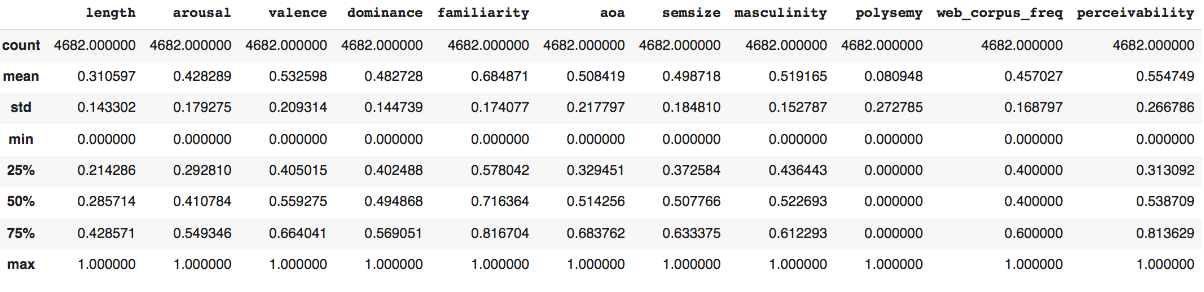
\includegraphics[width=0.8\textwidth]{stat2.png}
    \caption{Statistical information of the dataset used in the cluster analysis}
    \label{tab:stat2}
\end{figure}


\subsubsection{Principal Component Analysis (PCA)}

In order to reduce the dimensionality of the variables to use in the cluster analysis, a Principal Component Analysis is performed. The variables are reduced to a dimension of 4682 rows x 2 columns.

\subsection{Clustering analysis by K-Means}
The first clustering algorithm that we analyzed is \textit{K-Means}. It is one of the best known clustering algorithms. It is a simple unsupervised learning algorithm that is used to solve clustering problems. It follows a simple procedure of classifying a given dataset into a number of clusters, defined by the letter \textit{k}, which is fixed beforehand. The clusters are then positioned as points and all observations or data points are associated with the nearest cluster, computed and adjusted. Then the process starts over using the new adjustments until a desired result is reached.

\subsubsection{Identifying the optimal number of clusters}
Since the number of clusters for this algorithm is fixed beforehand, it becomes essential to identify the optimal quantity of clusters. This task can be done in a variety of ways.

For instance, one option is an empirical one, which is to try various number of clusters and then look for the best one. Another one is the \textit{Elbow method}, that looks at the total WSS (\textit{Within Cluster Sums of Squares}, the sum of distances between the points and the corresponding centroids for each cluster) as a function of the number of clusters: one should choose a number of clusters so that adding another cluster does not improve much the total WSS. The total WSS measures the compactness of clustering and ideally it should be as small as possible. 

Finally, the approach we chose is the \textit{Average Silhouette Method}. It measures the quality of a cluster, i.e. it determines how well each object lies within its cluster. A high average silhouette width indicates a good clustering. It computes the average silhouette of observations for different values of k. The optimal number of clusters k is the one that maximizes the average silhouette over a range of possible values for k\cite{books/wi/KaufmanR90}.

After the computation (the initial number of clusters is 2 and the final is 50), the result is that the ideal number of clusters for \textit{K-Means} is 3, as shown in Figure \ref{fig:Average silhouette score}.

\begin{figure}[h]
    \centering

\begin{minipage}{0.49\textwidth}
    \centering
    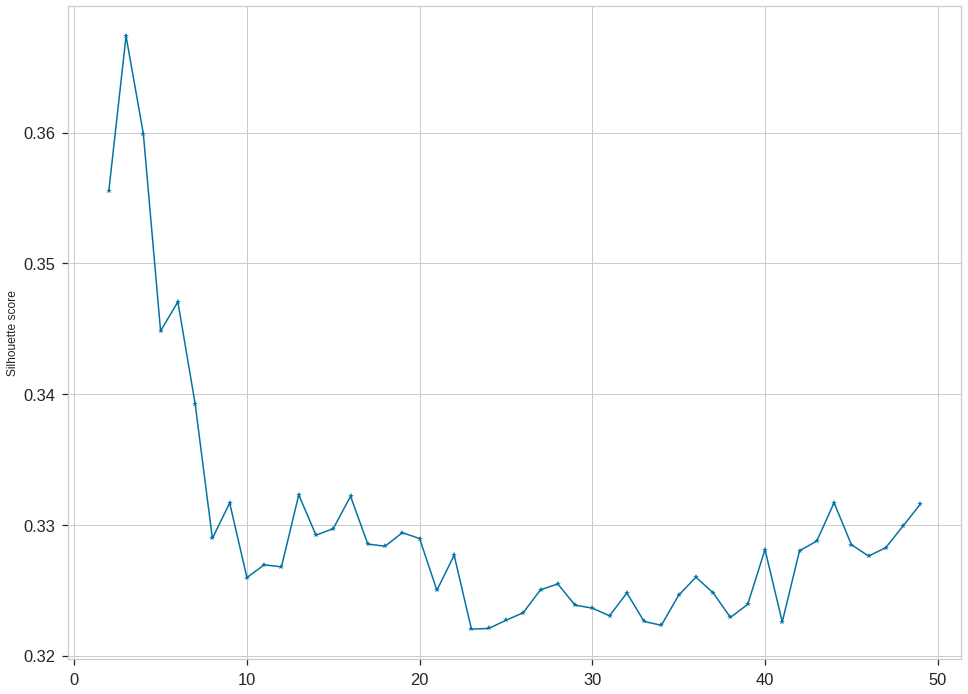
\includegraphics[width=0.7\textwidth]{Graphs/Average silhouette score.png}
    \caption{Average silhouette score}
    \label{fig:Average silhouette score}
\end{minipage}
\hfil
\begin{minipage}{0.5\textwidth}
\centering
    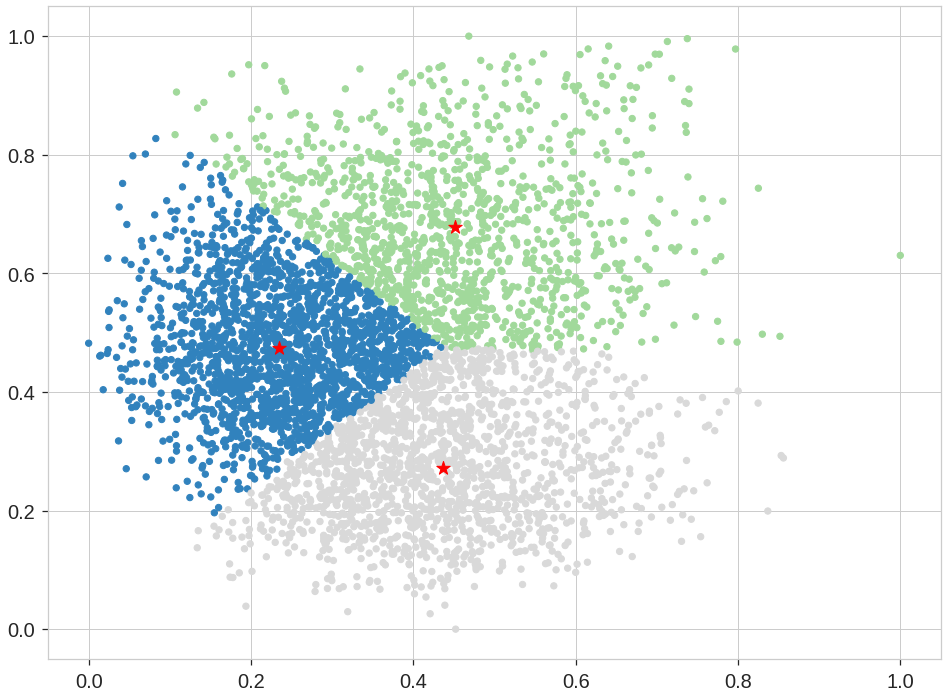
\includegraphics[width=0.7\textwidth]{Graphs/K-Means.png}
    \caption{K-Means clustering}
    \label{fig:K-Means}
\end{minipage}
%\caption{Plots used for the analysis of the K-Means algorithm}
\end{figure}

The value of the Silhouette score varies from -1 to 1. If the score is 1, the cluster is more dense and well-separated than other clusters. A value near 0 represents overlapping clusters with samples very close to the decision boundary of the neighboring clusters. A negative score [-1, 0] indicates that the samples might have got assigned to the wrong clusters. In this case, the highest value (closest to 1) is given by 3 clusters: 0.37.

\subsubsection{Clusters and results}
Finally, after calculating the best possible number of cluster to use for \textit{K-Means}, it is possible to compute the algorithm. The three clusters with their relative centroid can be seen in Figure \ref{fig:K-Means}.

\subsection{Analysis by Density-Based Clustering}
Density-based clustering locates regions of high density that are separated from one another by regions of low density. In this case, density is defined with the center-based approach, where it is estimated for a particular point in the dataset by counting the number of points within a specified radius $\varepsilon$ of that point. This allows to classify a point as \textbf{core} point if it falls withing the interior of a dense region, \textbf{border} point if on the edge of a dense region, or finally as a \textbf{noise} point if in a sparsely occupied region.

DBSCAN (\textit{Density-Based Spatial Clustering of Applications with Noise}) is a simple yet effective density-based clustering algorithm, it is one of the most common clustering algorithms, and operates as follows: any two core points that are close enough—within a distance $\varepsilon$ of one another are put in the same cluster. Likewise, any border point that is close enough to a core point is put in the same cluster as the core point. Ties need to be resolved if a border point is close to core points from different clusters. Noise points are discarded.

Being density-based, it is resistant to noise and can handle clusters of arbitrary shapes and sizes. Thus, DBSCAN can find many clusters that could not be found using K-means.

\subsubsection{Identifying the value of $\varepsilon$ and MinPts}
The basic approach is to look at the distance from a point to its kth nearest neighbor, which is called the k-dist. If we compute the k-dist for all the data points for some k, sort them in increasing order, and then plot the sorted values, we expect to see a sharp change at the value of k-dist that corresponds to a suitable value of $\varepsilon$. This behavior is well seen in Figure \ref{fig:eps}. If we select this elbow point as the $\varepsilon$ parameter and take the value of k as the MinPts parameter, then 
\begin{itemize}
    \item points for which k-dist is less than $\varepsilon$ will be labeled as core points;
    \item  other points will be labeled as noise or border points.
\end{itemize}

Given the dimension $d$ of the dataset, the value of k should be close to the double of $d$\cite{Sander1998}. 

For this particular dataset, the ideal value of distance is located at around $\varepsilon\approx 0.02$, which is the point of maximum curvature. It represents the optimization point where diminishing returns are no longer worth the additional cost, since increasing the number of clusters will improve the fit of the model, but could also increase the risk of overfitting. To estimate more accurately $\varepsilon$, we varied its value between 0.012 and 0.026 with a step of 0.001, as seen in Figure \ref{fig:vareps}. 

In the end, it was decided to set on $\varepsilon= 0.018$ and MinPts = 20, for a total of 11 cluster, not counting the noise. The results of the clustering can be seen in Figure \ref{fig:dbscan}.

\begin{figure}[h]
\centering
    \begin{minipage}[b]{.4\linewidth}
    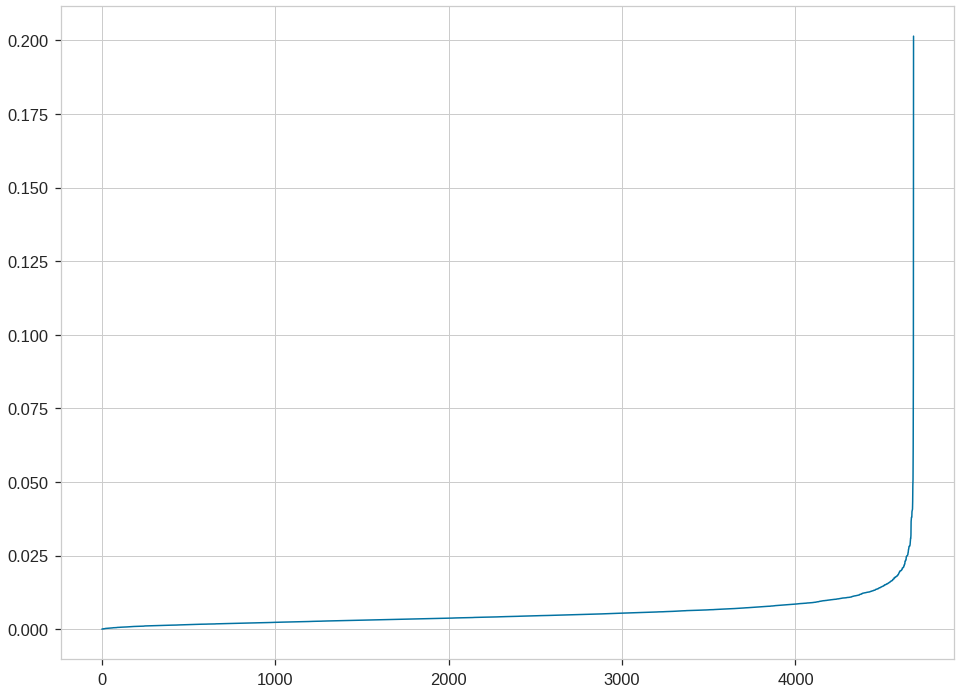
\includegraphics[width=\textwidth]{kth_neighbors.png}
    \caption{Points sorted by k-distance}
    \label{fig:eps}
    \end{minipage}
    \hfil
    \begin{minipage}[b]{.59\linewidth}
    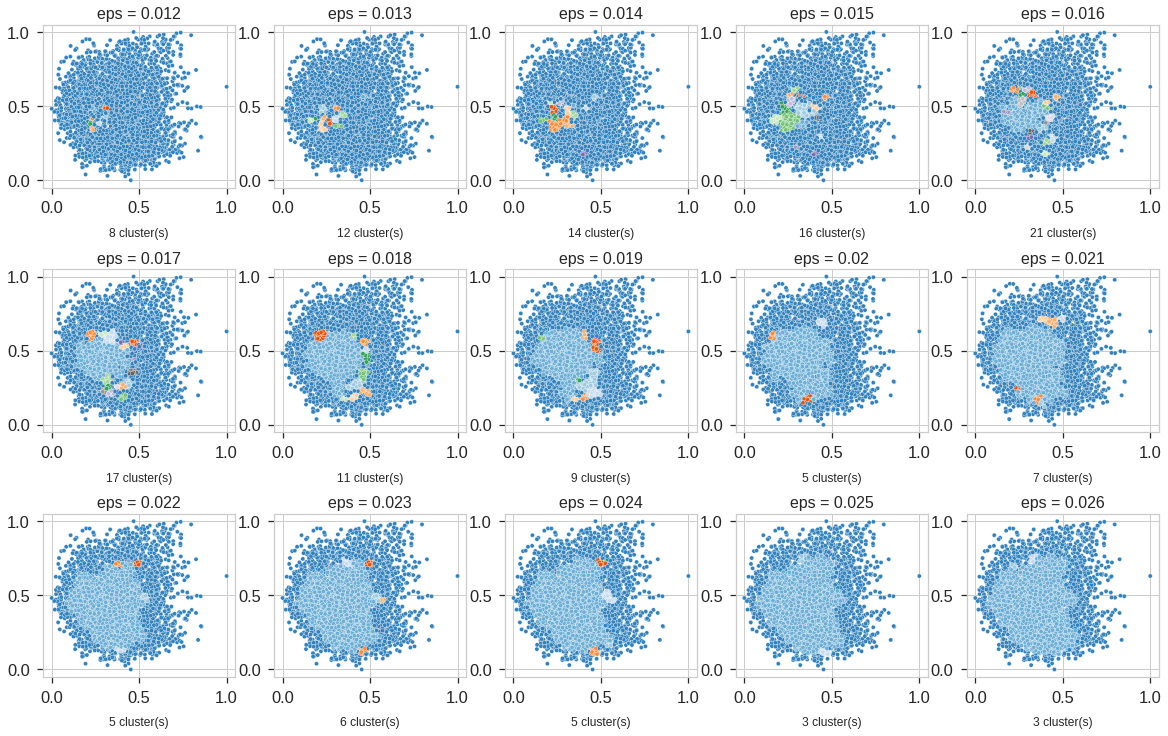
\includegraphics[width=\textwidth]{dibi.png}
     \caption{DBSCAN varying $\varepsilon$ between 0.012 and 0.026}
    \label{fig:vareps}
    \end{minipage}
\end{figure}

%\begin{figure}[h]
    %\centering
    %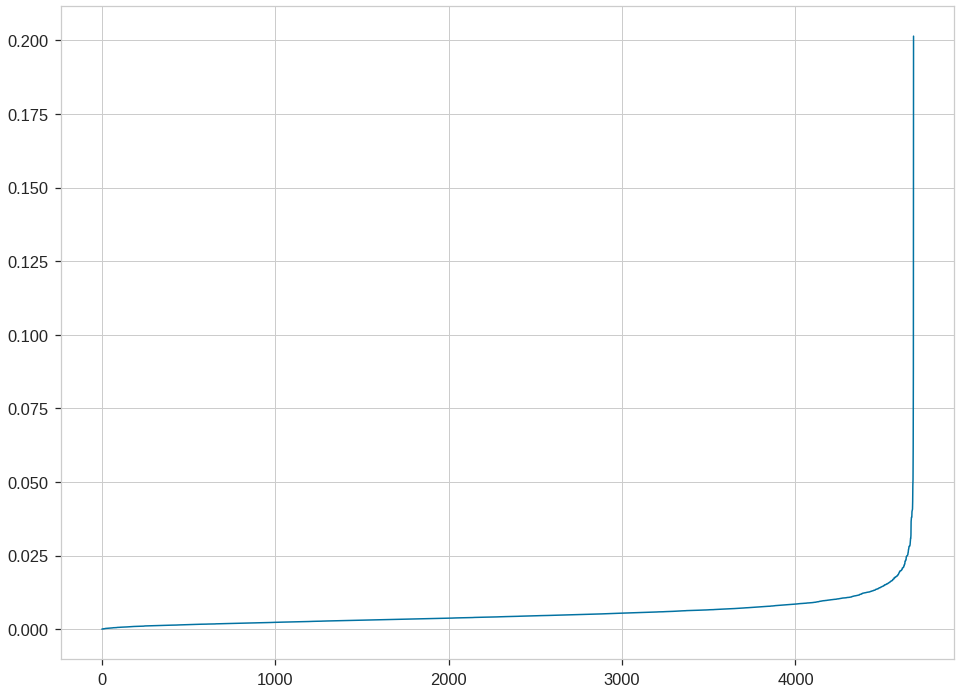
\includegraphics[width=8cm]{kth_neighbors.png}
    %\caption{Points sorted by distance to the 20th nearest neighbor to find optimal eps}
    %\label{fig:eps}
%\end{figure}

%\begin{figure}[h]
    %\centering
    %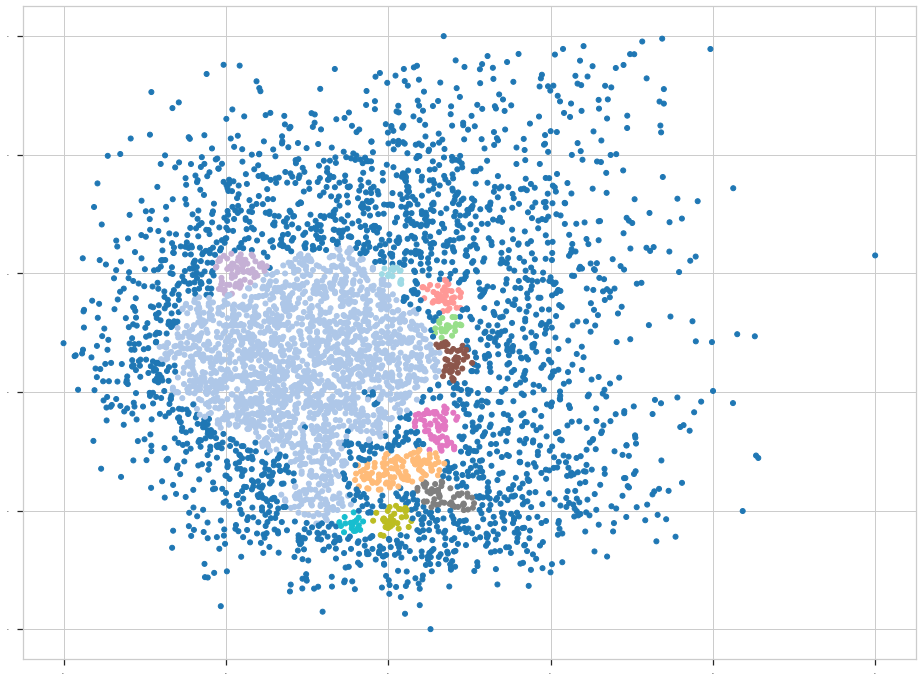
\includegraphics[width=10cm]{dbscan.png}
    %\caption{DBSCAN clustering}
   % \label{fig:dbscan}
%\end{figure}

\begin{figure}[h]
    \centering
    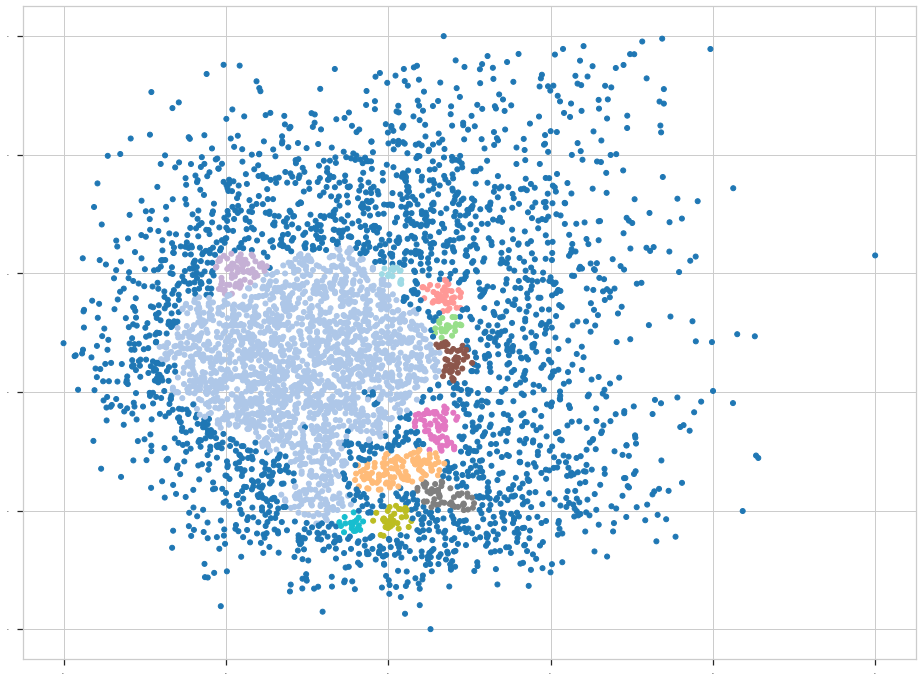
\includegraphics[width=0.4\textwidth]{dbscan.png}
    \caption{DBSCAN with $\varepsilon= 0.018$ and MinPts = 20: 11 cluster in total}
    \label{fig:dbscan}
\end{figure}

\subsection{Analysis by Hierarchical Clustering}
Hierarchical clustering is a group of unsupervised learning algorithms that merge or split the clusters in sequence. This process can be visualized in a diagram structured as a tree, the \textit{dendrogram}. 

The agglomerative techniques are the most common: at first, each point represents a single cluster and then, step by step, the clusters are merged according to the distance between them. In particular, we chose the Euclidean distance. 

The distance can be defined with different criteria: 
\begin{itemize}
    \item \textit{Min} or \textit{Single linkage} computes the proximity between the closest two points in different clusters;
    \item \textit{Max} or \textit{Complete linkage} measures the distance between the farthest points in different clusters;
    \item \textit{Group Average} computes the average of pairwise proximity between points in the clusters;
    \item \textit{Ward's method} minimizes the total within-cluster variance.
\end{itemize}

\subsubsection{Identifying the linkage criterion and the number of clusters}
 In Figure \ref{fig:dends}, we can see the \textit{dendrograms} generated by the different methods.

\begin{figure}[h!]
\begin{minipage}[b]{.25\linewidth}
    \centering
    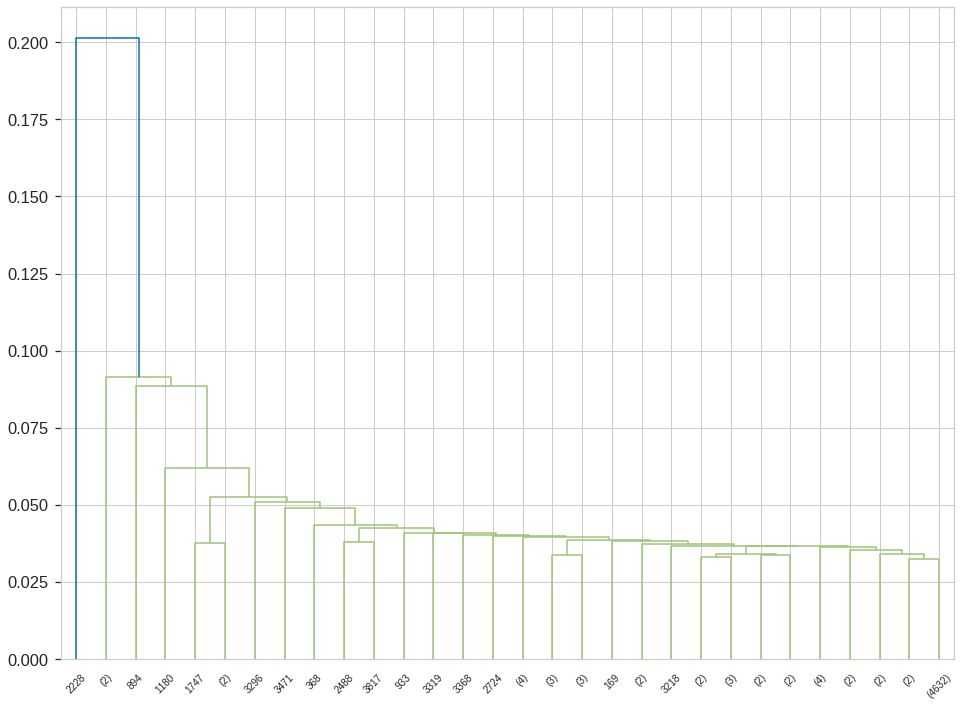
\includegraphics[width=\textwidth]{Graphs/h_single.png}\label{fig:MIN_dend}
    \subcaption{Single Link}
    \end{minipage}\hfill
    \begin{minipage}[b]{.25\linewidth}
    \centering
    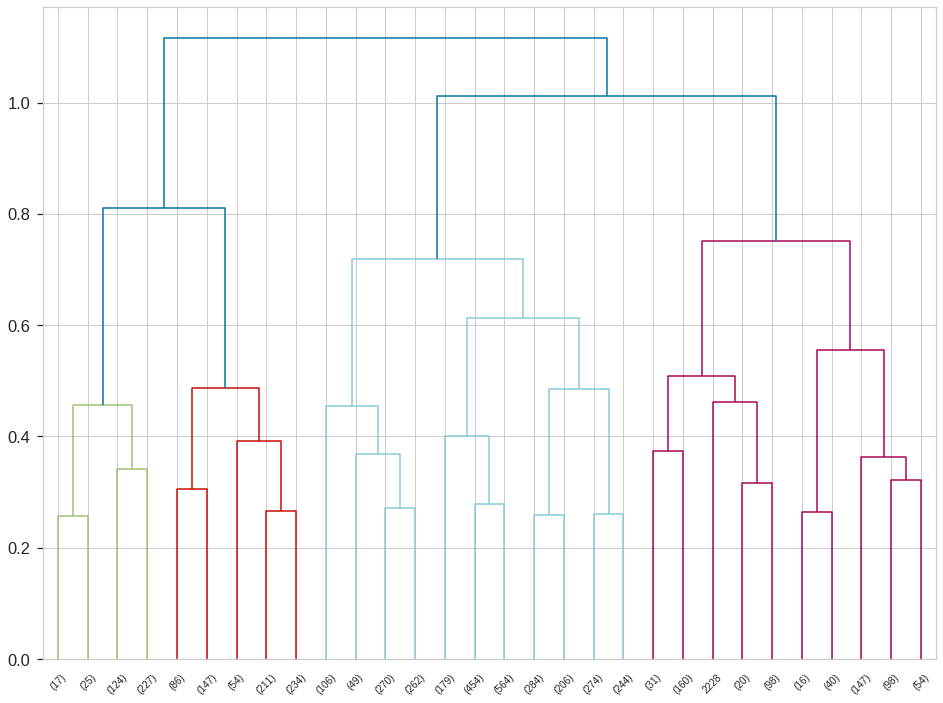
\includegraphics[width=\textwidth]{Graphs/h_complete.png}\label{fig:MAX_dend}
    \subcaption{Complete}
    \end{minipage}\hfill
    \begin{minipage}[b]{.25\linewidth}
    \centering
    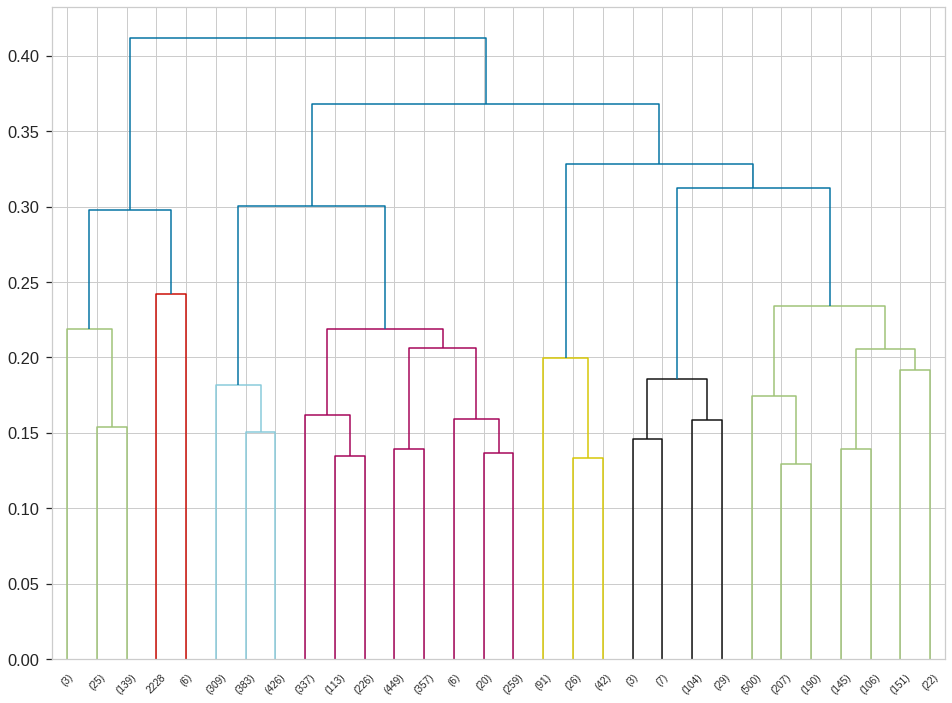
\includegraphics[width=\textwidth]{Graphs/h_average.png}\label{fig:avg_dend}
    \subcaption{Average}
    \end{minipage}\hfill
    \begin{minipage}[b]{.25\linewidth}
    \centering
    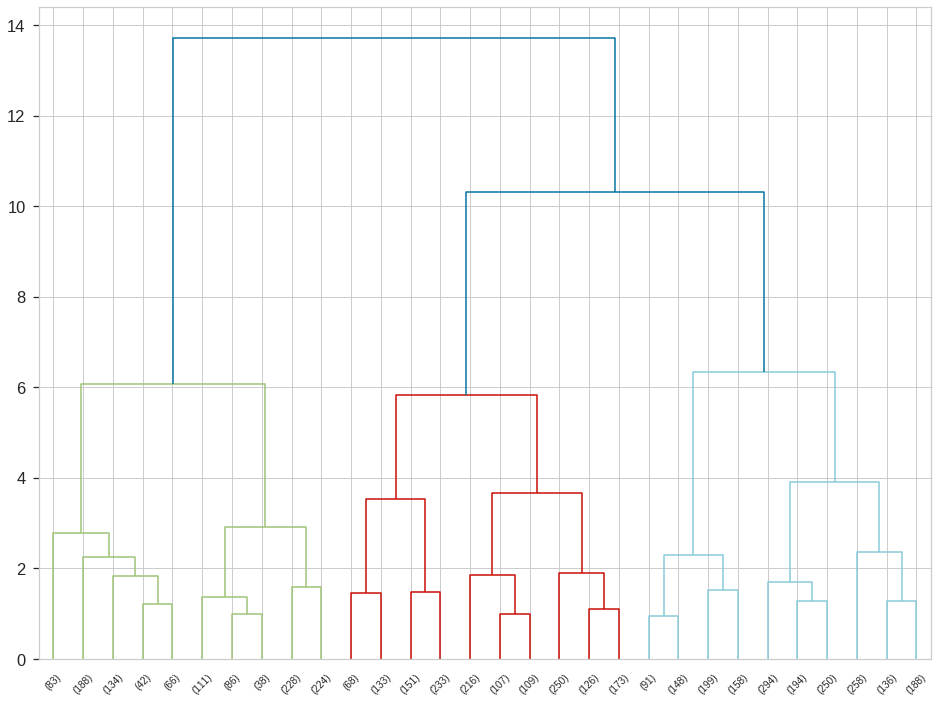
\includegraphics[width=\textwidth]{Graphs/h_ward.png}\label{fig:Ward_dend}
    \subcaption{Ward}
    \end{minipage}\hfill
    \caption{Dendrograms} \label{fig:dends}
\end{figure}


The \textit{dendograms} show that the \textit{Single Link} method gives us the worst result, with one big cluster that includes the majority of the points (regardless of the number of clusters we set), whereas \textit{Complete} and \textit{Average} linkage are more balanced. As expected, however the most balanced is \textit{Ward's method}, given the nature of the algorithm. 
 
 \textit{Single Link} method does not give much information, while \textit{Ward's Method} leads to a very similar analysis as that of K-Means. For this reason we decided to plot the scatterplot of the \textit{Complete} and \textit{Average} linkage, choosing respectively to cut at 6 and 7 clusters.
 
 The results of the clustering can be seen in Figure \ref{fig:hierach}.
 
\begin{figure}[h]
    \centering
    \begin{minipage}{0.49\textwidth}
    \centering
        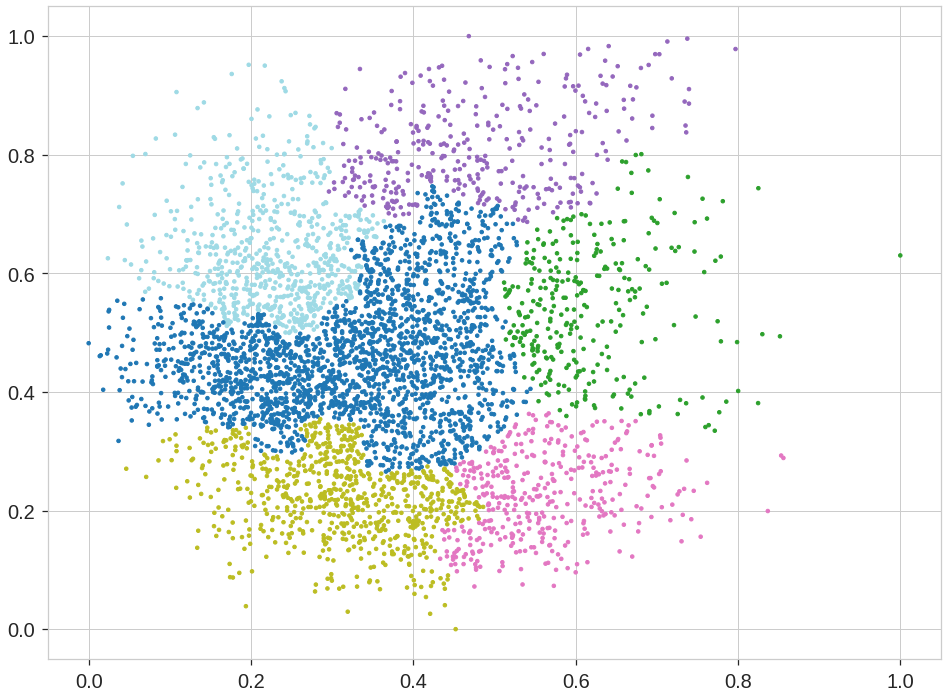
\includegraphics[width=0.65\textwidth]{complete.png}
\subcaption{Complete Linkage}
    \end{minipage}
    \hfill
        \begin{minipage}{0.49\textwidth}
        \centering
        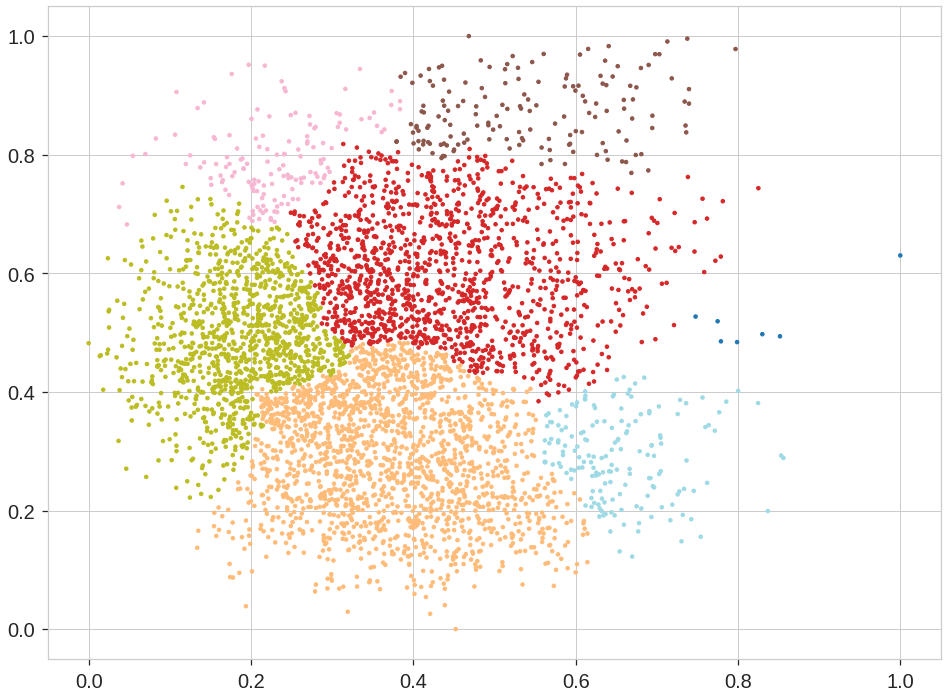
\includegraphics[width=0.65\textwidth]{average.png}
\subcaption{Average Linkage}
    \end{minipage}
    \caption{Hierarchical Clustering}
    \label{fig:hierach}
\end{figure}


\subsection{Final Discussion}

To validate each cluster algorithm, we decided to use two different test scores:
\begin{itemize}
    \item the \textbf{Silhouette Score:} it estimates the distances between clusters and provides a number between -1 and 1. Whereas: \textbf{1} means that the clusters are well apart from each other and clearly distinguished; \textbf{0} means that the clusters are indifferent, or we can say that the distance between clusters is not significant; \textbf{-1} means that the clusters are assigned in the wrong way.
    %\begin{itemize}
    %\item[] 
    %\end{itemize}
    \item \textbf{Calinski-Harabasz (Variance Ratio Criterion):} is the ratio of the sum of between-clusters dispersion and of inter-cluster dispersion for all clusters, the higher the score, the better the performances.
\end{itemize}

As a drawback, both the test scores are generally higher for convex clusters than other concepts of clusters, such as density based clusters like those obtained through DBSCAN. The scores for the clusters are tabulated in Table \ref{tab:scores}.

\begin{table}[h]
    \centering
    \adjustbox{max width=0.6\textwidth}{%
    \begin{tabular}{r|c|c|c}
    Evaluation scores & K-Means & DBScan & Hierarchical \\
    \hline
        \textbf{Silhouette:} & 0.36 & -0.34 & 0.21  \\
         \textbf{Calinski-Harabasz:} & 3575.89 & 59.95 & 2074.84
    \end{tabular}
    }
    \caption{Evaluation of different test scores for the type of analyzed cluster algorithms}
    \label{tab:scores}
\end{table}

According to the values in the Table \ref{tab:scores}, K-Means has the best scores among the three algorithms. But we have to take into consideration that the high value of the coefficients for the K-Means algorithm may be biased due to the low number of clusters used (i.e. 3).
\begin{figure}[h]
    \begin{minipage}{0.47\linewidth}
            \centering
            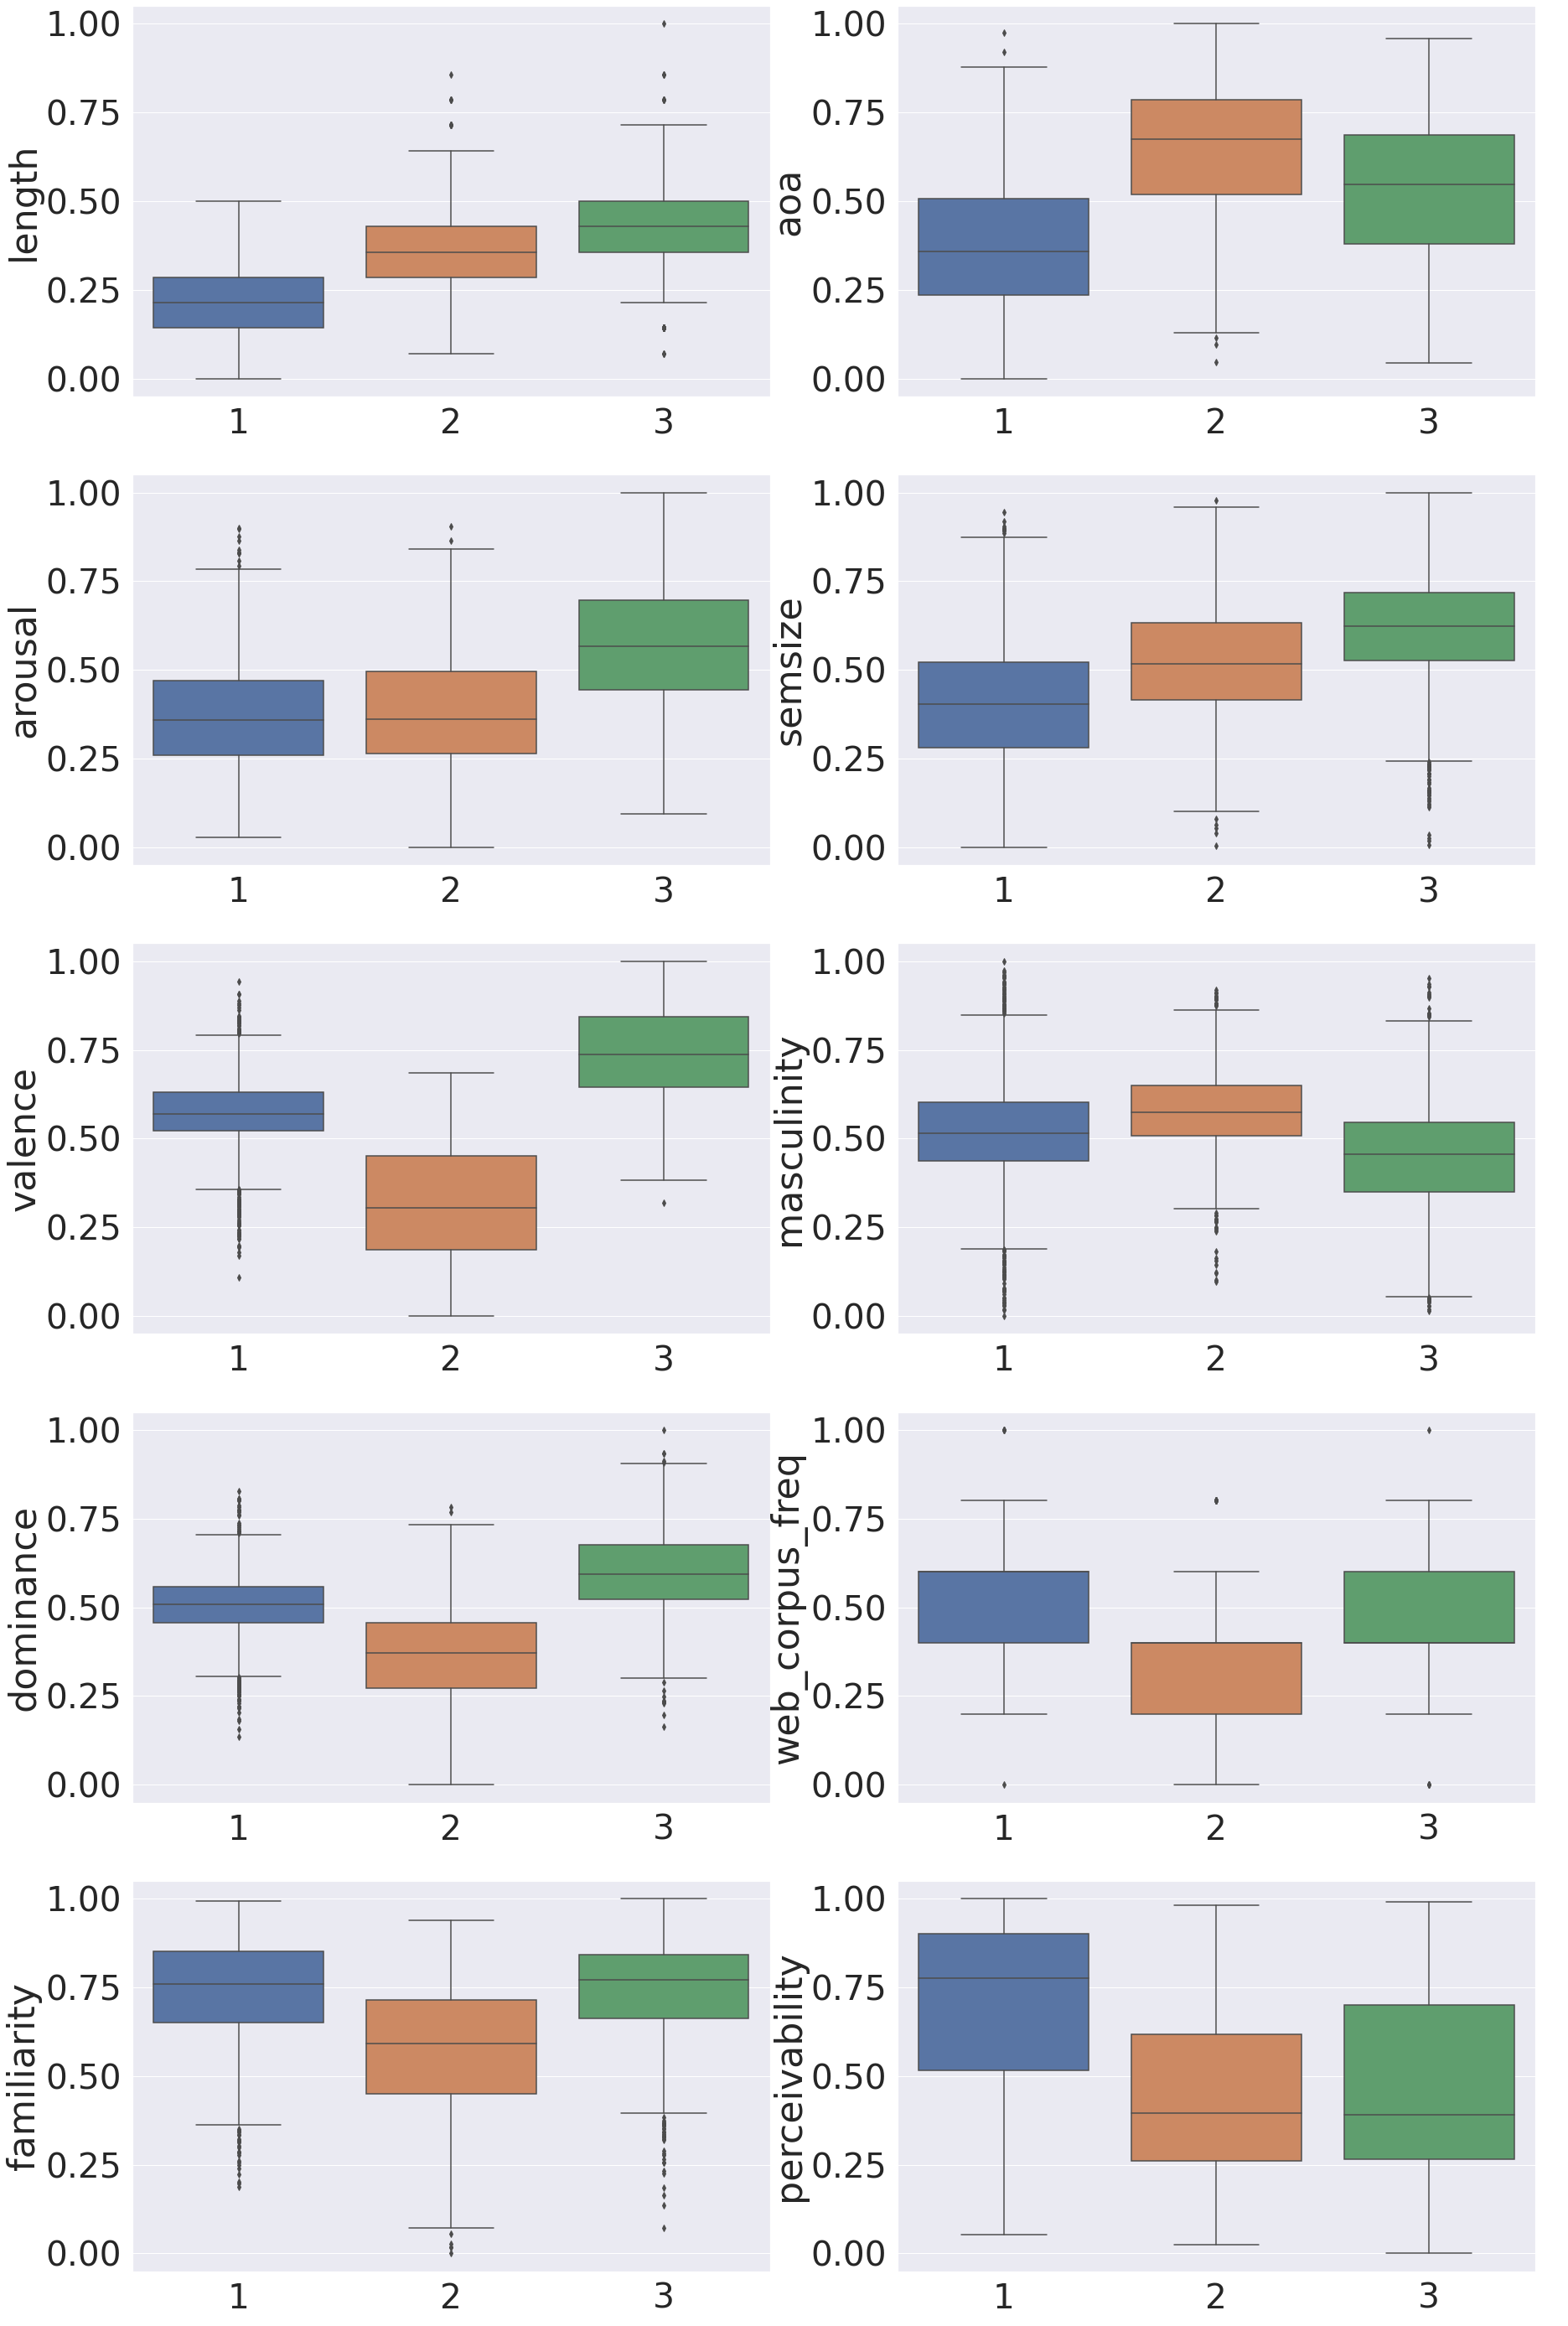
\includegraphics[width=0.8\textwidth]{kmeans-box2.png}
            \subcaption{K-Means}\label{fig:boxclukmeans}
    \end{minipage}
    \hfil
    \begin{minipage}{0.47\linewidth}
            \centering
            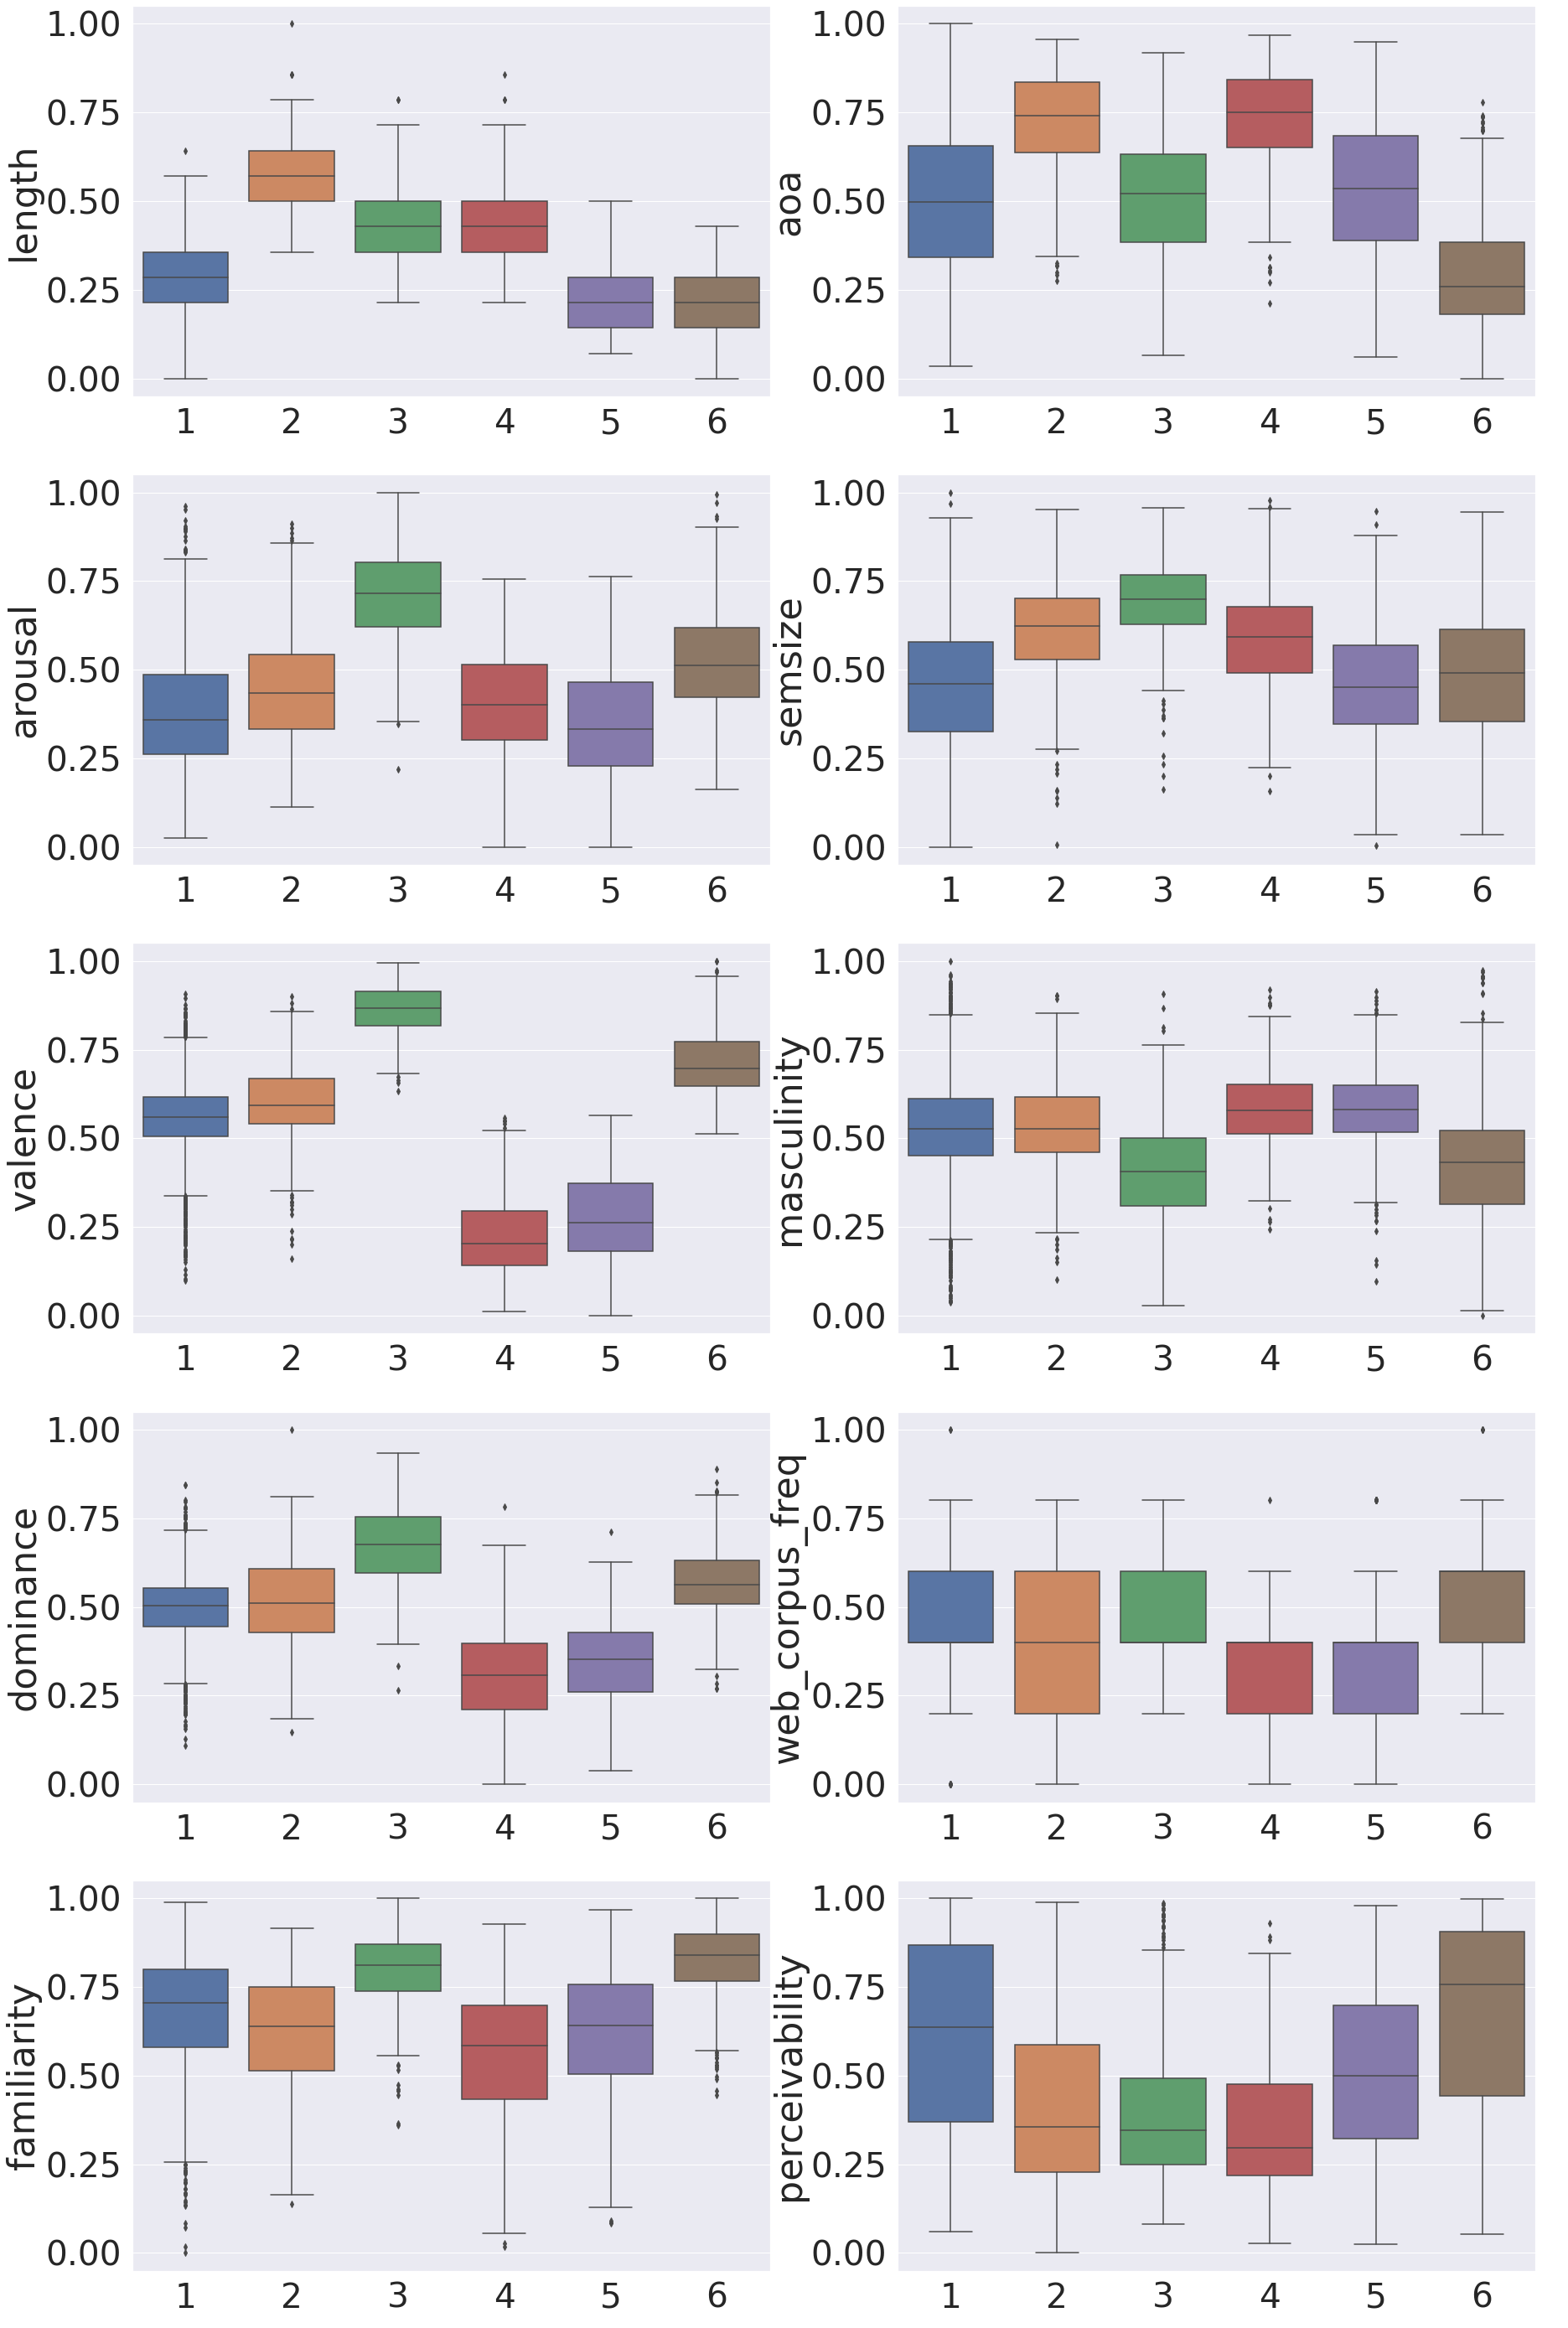
\includegraphics[width=0.8\textwidth]{hierarchical-box2.png}
            \subcaption{Hierarchical}\label{fig:boxcluhier}
    \end{minipage}
        \caption{Boxplots of variables for two cluster algorithms}
    \label{fig:boxcluster}
\end{figure}


Additionally, one can perform an analysis by looking at the boxplots of the variables according to the assigned cluster. The obtained results are showed in Figure \ref{fig:boxcluster}.


This kind of analysis is useful to determinate some key characteristics of the clusters. 

For instance, in the K-Means analysis (Fig. \ref{fig:boxclukmeans}) the Second cluster has a low value for \textit{Web Corpus Freq}, high value for \textit{AoA}, and low value for \textit{Familiarity}. This indicates that the words that belong to this cluster may be difficult words, and for that reason they are not commonly used. To cross check this analysis one can see some words of this cluster (e.g. \textit{abbey}, \textit{zeal}), which confirm this hypothesis.
Some of these words are classified by the Hierarchical Clustering (Figure \ref{fig:boxcluhier}) algorithm in the Fourth cluster, which has similar characteristics to the Second cluster of K-Means.

Conversely, the words of the Third Cluster of Hierarchical Clustering have high valence, high dominance, high semsize and low perceivability. These properties may indicate that this cluster contains words that convey a high (emotional) impact. Finally, the Sixth cluster may represent words that are easy, short and acquired in early age.


\section{Classification}

The classification task was performed using three different methods, which will be described in following sections. Before that, we briefly expose the data preprocessing used for this analysis.  

\subsection{Preprocessing}

Similarly to the cluster section, we decided to use our transformed dataset, described in Figure \ref{tab:stat2}. 

However, for the classification process the parameters excluded from the normalization are \textit{length} and \textit{web\_corpus\_frequency}, which remain discrete.

Once chosen, the target variable is removed from the dataset and stored in another array. The choice and handling of this variable is described in section \ref{target_dt}. It is also necessary to split the dataset in a training and a testing set, respectively 70\% and 30\% of the total, which remain the same for the three analyzed algorithms.

\subsection{Decision Trees}\label{sec:decisio-tree}\label{sec:building_tree}

According to the scikit-learn documentation, Decision Trees (DTs) are a \textit{non-parametric supervised learning method used for classification and regression}\cite{JMLR:v12:pedregosa11a}. The goal is to create a model that predicts the value of a target variable by learning simple decision rules inferred from the data features.

\begin{figure}[h]
\begin{minipage}{0.7\linewidth}
        \centering
    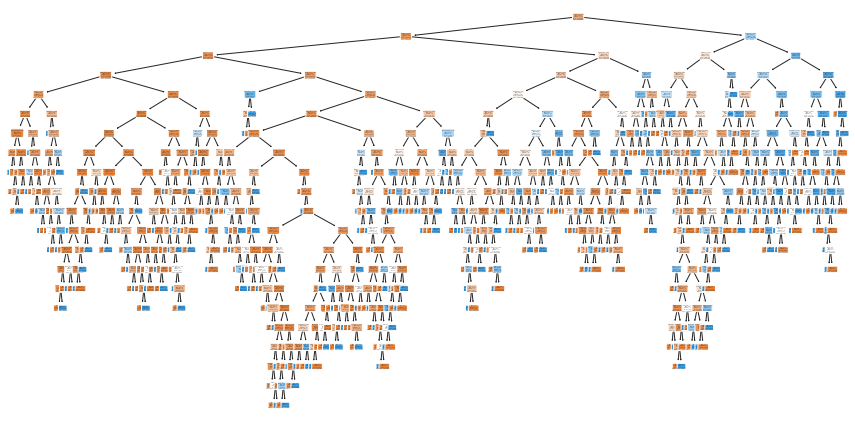
\includegraphics[width=0.9\textwidth]{overfit_tree_arousal.png}
    \subcaption{Overfitted tree}
    \label{fig:overfit_tree}
\end{minipage}
\hfill
    \begin{minipage}{0.3\linewidth}
            \centering
            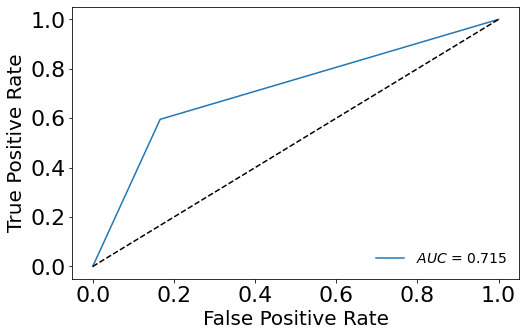
\includegraphics[width=0.9\textwidth]{arousal_overfit_ROC.png}
            \subcaption{ROC curve for the testing set}\label{overroc}
    \end{minipage}
    \caption{Unpruned tree and ROC for target variable \textit{arousal}}\label{overfit}
\end{figure}

If we build the tree in a naive way, using the algorithm with the default parameters (Gini impurity measure, max\_depth=0, etc...), we obtain a very complex tree (Figure \ref{fig:overfit_tree}). This tree is overfitted and therefore does not perform well on the testing set, as seen in the ROC curve in Figure \ref{overroc}.

To avoid this behavior, we can introduce the parameter \textit{Cost Complexity Pruning} (CCP) $\alpha$, which prevent the tree from overfitting. This parameter is particularly useful because the tuning of the other parameters (\textit{Max Depth}, \textit{Min Samples Leaf}, etc.) is not necessary anymore.

The choice of the value of the parameter $\alpha$ is determined by varying it over several attempts and calculating the tree score for the training set as well as the testing set, as shown in Figure \ref{fig:alpha_accuracy}. To avoid statistical errors, the whole process is repeated, performing a 10-fold cross validation. Finally, the mean accuracy value for the testing and training set is calculated with a 10-fold cross validation varying $\alpha$, as shown in Figure \ref{fig:mean_accuracy}.

\begin{figure}[h]
\begin{minipage}{0.5\linewidth}
        \centering
    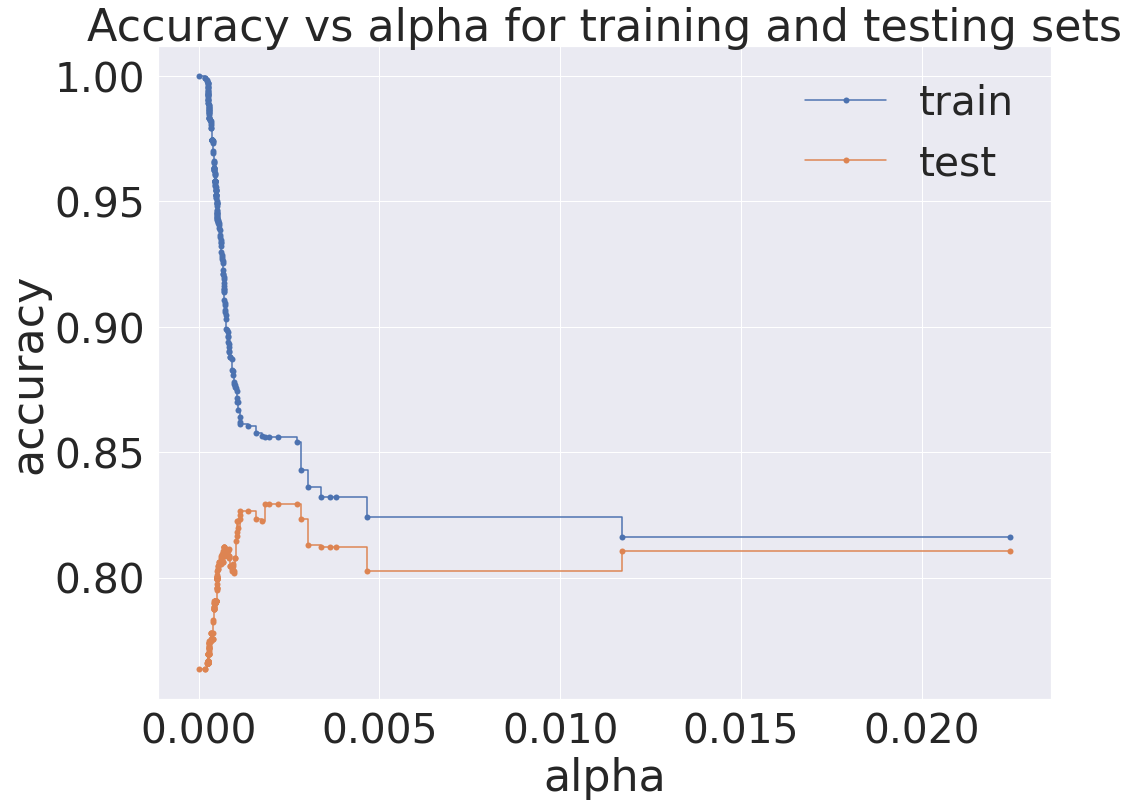
\includegraphics[width=0.8\textwidth]{accuracy_vs_alpha.png}
    \subcaption{Plot of accuracy vs $alpha$ for 1-fold validation}
    \label{fig:alpha_accuracy}
\end{minipage}
\hfill
    \begin{minipage}{0.5\linewidth}
        \centering
    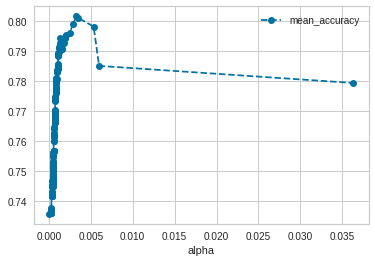
\includegraphics[width=0.8\textwidth]{mean_accuracy.png}
    \subcaption{Mean accuracy vs $alpha$ for 10-fold validation}
    \label{fig:mean_accuracy}
\end{minipage}
    \caption{Plots for the cost complexity pruning}
\end{figure}

Based on these results, we choose the $\alpha$ that maximizes the accuracy and we build a new pruned tree using this parameter. As shown in Figure \ref{fig:pruned_ccp}, the new tree is simpler and performs better.

\begin{figure}[h]
\centering
\begin{minipage}{0.49\linewidth}
    \centering
    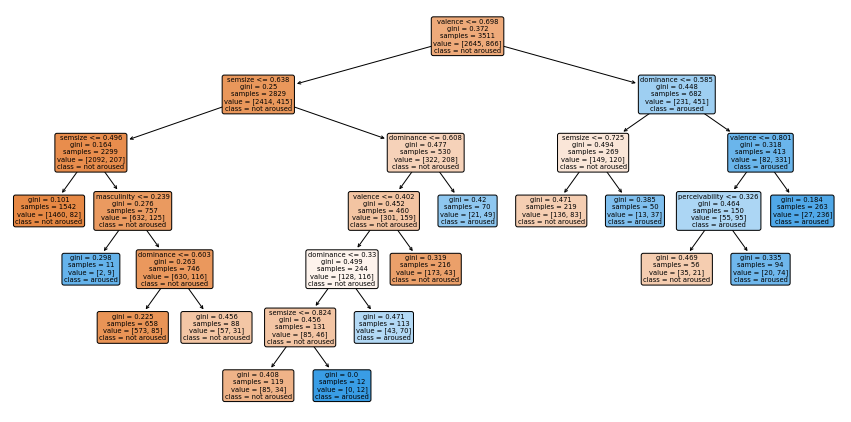
\includegraphics[width=\textwidth]{pruned_tree_arousal.png}
    \subcaption{CCP}
    \label{fig:pruned_ccp}
    \end{minipage}\hfil
    \begin{minipage}{0.48\linewidth}
    \centering
    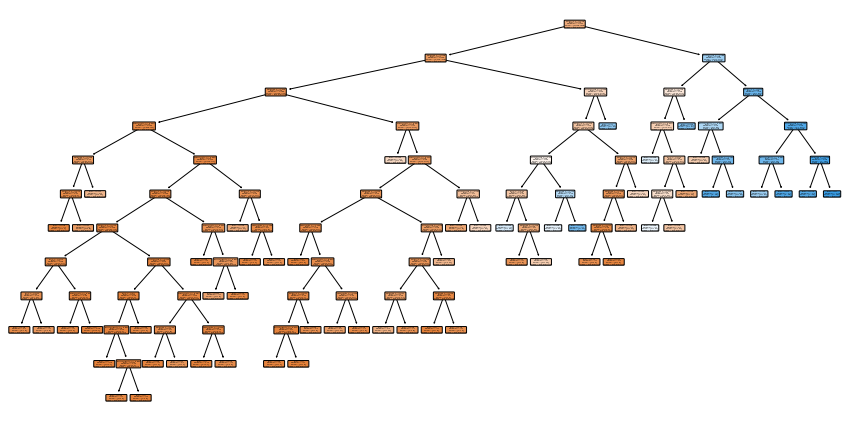
\includegraphics[width=\textwidth]{pruned_tree_citraro.png}
    \subcaption{Grid Search}
    \label{fig:pruned_grid}
    \end{minipage}
    \caption{Pruned Trees}
\end{figure}
This analysis is performed with both the \textit{gini} and \textit{entropy} impurity measures. The results obtained with this classification algorithm will be discussed in the following sections.

An alternative to this method is a \textit{grid search} for the best parameters (\textit{Max Depth, Min Samples Split, Min Samples Leaf}) using the F1 score as measure. With the grid search, the accuracy and the other test scores obtained are similar to the ones for CCP, but the complexity of the tree is higher, as shown in Figure \ref{fig:pruned_grid}. For this reason we opted for the cost complexity pruning method, tuning the parameter $\alpha$.




\subsection{Random Forest}

Decision Trees are a useful tool for classification because of their simplicity, but they present problems when it comes to classifying a new set. An improvement of this algorithm may be the Random Forest. This method consists in creating different bootstrapped datasets from the training sets and creating for each one a decision tree (more generally, an \textit{estimator}), as described in section \ref{sec:decisio-tree}, without tuning the parameters. Then, each record will be evaluated by every tree (a.k.a. by the \textit{forest}) and classified according to the majority of the outputs.

To determine the number of estimators we run different simulations and pick the value with the lowest \textit{Out Of Bag error}, i.e. the misclassification error on the records that did not enter the bootstrapped dataset.

%We applied Random Forest on the most interesting variables, as mentioned above: \textit{Valence}, \textit{Polysemy} and \textit{Age of Acquisition}. 
Taking the confusion matrices and the scores table into consideration, the results will be commented in the conclusion section.


\subsection{K - Nearest Neighbors}
The last classification algorithm we used is K-Nearest Neighbors (KNN). With this method, the target variable is classified by the majority of votes of its $k^{th}$ neighbors. If, for example, the majority of neighbors of a new record belong to class 1, the new item will be classified as 1 as well.  

%KNN works by firstly i.e. "classification is computed from a simple majority vote of the nearest neighbors of each point: a query point is assigned the data class which has the most representatives within the nearest neighbors of the point."\cite{JMLR:v12:pedregosa11a}. 

%We applied KNN on the fore mentioned variables: \textit{Valence}, \textit{Polysemy} and \textit{Age of Acquisition}. 
To determine optimal k, we iterate the algorithm for each variable over several values of k and pick the one that maximizes the accuracy. The most accurate value for k depends on the target variable. The results will be commented in the next sections.



\subsection{Choice of target variable}\label{target_dt}

The provided dataset is not meant to have a specific target variable. For that reason, we perform the analysis described in the previous sections for every single parameter. We decided to divide them into \textit{binary} and \textit{multi-split} target variables. 

\paragraph{Binary target variables} are obtained from continuous variables by setting a threshold. The values under the threshold are labeled as 0, while those above are labeled as 1. The thresholds for each variable are chosen according to the last quartile. We report the values of the thresholds in Table \ref{tab:threshold}.

\begin{table}[h]
\adjustbox{max width=\textwidth}{%
    \centering
    \begin{tabular}{|r|c|c|c|c|c|c|c|c|c|}
    \hline
        & Arousal & Valence & Dominance & Familiarity & Size & Masculinity & Polysemy & Perceivability & Aoa\\\hline
        \textbf{Threshold} & 0.55 & 0.67 & 0.57 & 0.60 & 0.63 & 0.60 & 0.50 & 0.80 & 0.60\\
        \hline
    \end{tabular}
    }
            \caption{Thresholds used for the binary split}\label{tab:threshold}
    \end{table}


The accuracy, precision, recall and F1 score of the Decision Tree using the \textit{entropy} criterion for each variable are shown in Table \ref{tab:class_scores}.

\begin{table}[h]
    \centering
\adjustbox{max width=\textwidth}{%
    \begin{tabular}{|r|c|c|c|c|c|c|c|c|c|}
    \hline
                    & Arousal & Valence & Dominance & Familiarity & Size & Masculinity & Polysemy & Perceivability & Aoa\\\hline\hline
        
        \textbf{Accuracy}             & 0.83 & 0.87 & 0.82 & 0.82 & 0.80 & 0.76 & 0.93 & 0.81 & 0.81\\\hline
        
        \textbf{Precision (0)}        & 0.85 & 0.79 & 0.87 & 0.71 & 0.82 & 0.85 & 0.93 & 0.84 & 0.83\\
        \textbf{Precision (1)}        & 0.75 & 0.89 & 0.66 & 0.85 & 0.66 & 0.52 & 0.00 & 0.68 & 0.79\\
        \textbf{Precision (wgt mean)} & 0.86 & 0.86 & 0.82 & 0.82 & 0.78 & 0.77 & 0.87 & 0.80 & 0.81\\\hline
        
        \textbf{Recall (0)}           & 0.94 & 0.94 & 0.89 & 0.58 & 0.92 & 0.82 & 1.00 & 0.90 & 0.89\\
        \textbf{Recall (1)}           & 0.52 & 0.67 & 0.61 & 0.91 & 0.44 & 0.58 & 0.0  & 0.55 & 0.69\\
        \textbf{Recall (wgt mean)}    & 0.87 & 0.87 & 0.82 & 0.82 & 0.80 & 0.76 & 0.93 & 0.81 & 0.81\\\hline
        
        \textbf{F1 score (0)}         & 0.89 & 0.91 & 0.88 & 0.64 & 0.87 & 0.84 & 0.96 & 0.87 & 0.86\\
        \textbf{F1 score (1)}         & 0.61 & 0.73 & 0.63 & 0.88 & 0.53 & 0.55 & 0.00 & 0.61 & 0.73\\
        \textbf{F1 score (wgt mean)}  & 0.86 & 0.86 & 0.82 & 0.82 & 0.78 & 0.76 & 0.90 & 0.80 & 0.81\\\hline
        
    \end{tabular}
    }
            \caption{Score values of DT for binary target variables, wheares the mean is weighted on the support.}\label{tab:class_scores}

    \end{table}
    
    
    Based on these results, we chose to focus our analysis on three variables. The most interesting one appears to be \textit{Valence}, given its high scores. In addition, we analyze \textit{Age of Acquisition} since the comparison with the multi-split analysis may be interesting. \textit{Polysemy} is a variable to considerate because it is already binary.
    
    The scores of Random Forest and KNN for these variables are shown in the Tables \ref{tab:rf_scores} and \ref{tab:knn_scores}, respectively. The number of k used in the KNN algoithm is 6 for \textit{Valence}, 6 for \textit{AoA} and 3 for \textit{Polysemy}.
    
Taking also into consideration the confusion matrices, the results will be commented in the conclusion section.
    
%Tabella con accuracy, f1 score, etc

\begin{minipage}{0.49\linewidth}
    \centering
    \begin{table}[H]

    \centering
    \begin{tabular}{|r|c|c|c|}
    \hline
        & Valence & Polysemy & Aoa\\\hline\hline
        
        \textbf{Accuracy} & 0.88 & 0.93 & 0.82\\\hline
        
        \textbf{Precision (0)} & 0.89 & 0.93 & 0.83\\
        \textbf{Precision (1)} & 0.85 & 0.33 & 0.80\\
        \textbf{Weighted mean} & 0.88 & 0.89 & 0.82\\\hline
        
        \textbf{Recall (0)} & 0.96 & 1.0 & 0.90\\
        \textbf{Recall (1)} & 0.67 & 0.01 & 0.68\\
        \textbf{Weighted mean} & 0.88 & 0.93 & 0.82\\\hline
        
        \textbf{F1 score (0)} & 0.92 & 0.96 & 0.86\\
        \textbf{F1 score (1)} & 0.75 & 0.02 & 0.74\\
        \textbf{Weighted mean} & 0.87 & 0.90 & 0.82\\\hline
        
    \end{tabular}
            \caption{Score values of Random Forest}\label{tab:rf_scores}
    \end{table}
    \end{minipage}
    \hfil
   \begin{minipage}{0.49\linewidth}
    \centering
        \begin{table}[H]

    \centering
    \begin{tabular}{|r|c|c|c|}
    \hline
        & Valence & Polysemy & Aoa\\\hline\hline
        
        \textbf{Accuracy} & 0.88 & 0.95 & 0.83\\\hline
        
        \textbf{Precision (0)} & 0.87 & 0.96 & 0.81\\
        \textbf{Precision (1)} & 0.92 & 0.70 & 0.88\\
        \textbf{Weighted mean} & 0.88 & 0.94 & 0.84\\\hline
        
        \textbf{Recall (0)} & 0.98 & 0.99 & 0.95\\
        \textbf{Recall (1)} & 0.58 & 0.38 & 0.63\\
        \textbf{Weighted mean} & 0.88 & 0.95 & 0.83\\\hline
        
        \textbf{F1 score (0)} & 0.92 & 0.97 & 0.87\\
        \textbf{F1 score (1)} & 0.71 & 0.49 & 0.73\\
        \textbf{Weighted mean} & 0.87 & 0.94 & 0.82\\\hline
        
    \end{tabular}
            \caption{Score values of KNN}    \label{tab:knn_scores}

    \end{table}
\end{minipage}


\paragraph{Multi-split target variables} are \textit{Web Corpus Frequency} and \textit{Age of Acquisition}. 

The variable \textit{Web Corpus Frequency} has already been discretized in the section \ref{discretize}.

The variable \textit{Age of Acquisition} can be seen as a discrete variable, truncating the original values. In this way, we obtain a binned parameter between 1 and 6, which represents the age in which the word was learned (as described in section \ref{semantic}).

Given the multi-output, the ROC curve is misdefined and for this reason we decided not to draw it. We report the Confusion Matrices directly in Figure \ref{aoa_multi}.

\begin{figure}[h]
  \begin{minipage}{.4\linewidth}
    \centering
    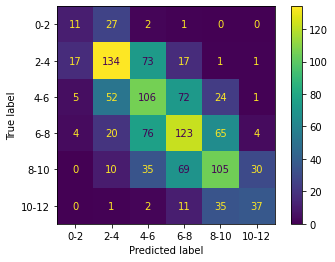
\includegraphics[width=\textwidth]{aoa_multi_confusion_matrix.png}%
  \end{minipage}
  \begin{minipage}{.2\linewidth}
    \centering

\begin{tabular}{|r|c|c|c|c|}
\toprule
{} &  \textbf{Precision} &    \textbf{Recall} &  \textbf{F1-Score} &      \textbf{Support} \\
\midrule\midrule
label 0-2     &   0.30 &  0.27 &  0.28 &    41 \\
label 2-4     &   0.55 &  0.55 &  0.55 &   243 \\
label 4-6     &   0.36 &  0.41 &  0.38 &   260 \\
label 6-8     &   0.42 &  0.42 &  0.42 &   292 \\
label 8-10    &   0.46 &  0.42 &  0.44 &   249 \\
label 10-12   &   0.51 &  0.43 &  0.47 &    86 \\\hline
%\textbf{macro avg}    &   0.43 &  0.42 &  0.42 &  1171 \\
\textbf{weighted avg} &   0.44 &  0.44 &  0.44 &  1171 \\
\textbf{accuracy}     &   0.44 &  0.44 &  0.44 &     0.44 \\
\bottomrule
\end{tabular}

  \end{minipage}
  
  \caption{Confusion Matrix and score values for Age of Acquisition} \label{aoa_multi}
\end{figure}

As seen in the Tables and more specifically in the confusion matrix of Figure \ref{aoa_multi}, these results are not really useful. The results for \textit{Web Corpus Frequency} are not reported because they were not found of interest, given their low accuracy.

Theoretically, the KNN algorithm performs well with multi-split target variable. The analysis for \textit{Age of Acquisition} performed with K=14 is summarized in Figure \ref{aoa_multi_KNN}.

\begin{figure}[h]
  \begin{minipage}{.4\linewidth}
    \centering
    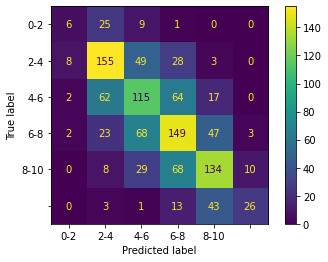
\includegraphics[width=\textwidth]{aoa_multi_knn_matrix.png}%
  \end{minipage}
  \begin{minipage}{.2\linewidth}
    \centering

\begin{tabular}{|r|c|c|c|c|}
\toprule
{} &  \textbf{Precision} &    \textbf{Recall} &  \textbf{F1-Score} &      \textbf{Support} \\
\midrule\midrule
label 0-2     &   0.33 &  0.15 &  0.20 &    41 \\
label 2-4     &   0.56 &  0.64 &  0.60 &   243 \\
label 4-6     &   0.42 &  0.44 &  0.43 &   260 \\
label 6-8     &   0.46 &  0.51 &  0.48 &   292 \\
label 8-10    &   0.45 &  0.54 &  0.54 &   249 \\
label 10-12   &   0.66 &  0.30 &  0.42 &    86 \\\hline
%\textbf{macro avg}    &   0.43 &  0.42 &  0.42 &  1171 \\
\textbf{weighted avg} &   0.50 &  0.50 &  0.49 &  1171 \\
\textbf{accuracy}     &   0.50 &  0.50 &  0.50 &     0.50 \\
\bottomrule
\end{tabular}


  \end{minipage}
  
  \caption{Confusion Matrix and score values for \textit{Age of Acquisition} multiplit with KNN} \label{aoa_multi_KNN}
\end{figure}

As predicted, we can see an improvement with respect to the Decision Tree classification method. However, the scores remain low and for this reason, the multi-target-variable analysis will not be discussed in the conclusions.

\subsection{Final Discussion}
The ROC and AUC of all the models applied to the binary variable are reported in Figure \ref{fig:roc}.
\begin{figure}[h]
\centering
\begin{minipage}[b]{.3\linewidth}
\centering\large 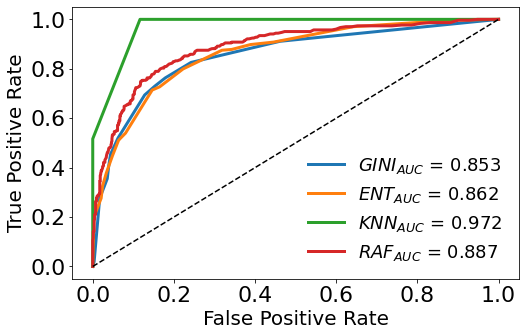
\includegraphics[width=0.8\linewidth]{arousal_ROC_c.png}
\subcaption{Arousal}\label{fig:arroc}
\end{minipage}%
    \hfil
\begin{minipage}[b]{.3\linewidth}
\centering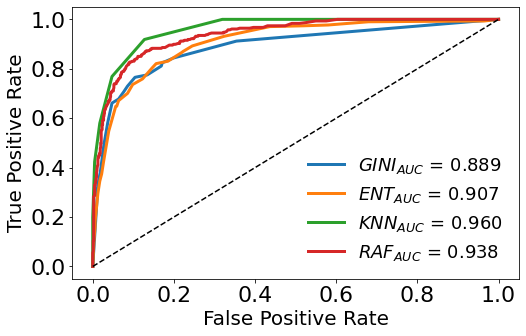
\includegraphics[width=0.8\linewidth]{valence_ROC_c.png}\subcaption{Valence}\label{fig:valroc}
\end{minipage}    \hfil
\begin{minipage}[b]{.3\linewidth}
\centering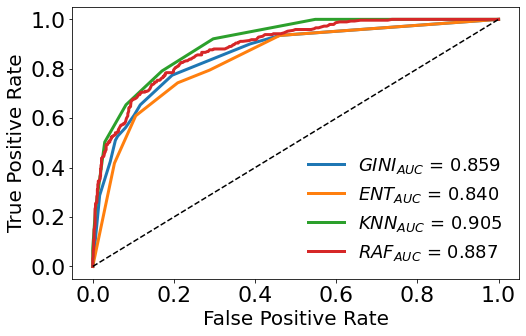
\includegraphics[width=0.8\linewidth]{dominance_ROC_c.png}\subcaption{Dominance}\label{fig:domroc}
\end{minipage}

\begin{minipage}[b]{.3\linewidth}
\centering\large 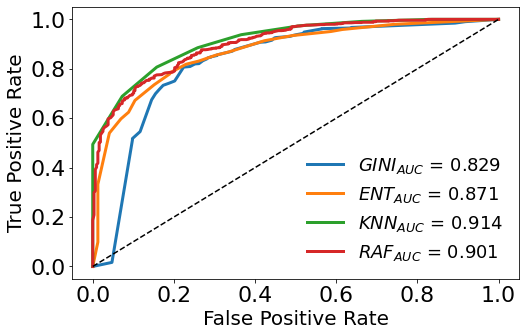
\includegraphics[width=0.8\linewidth]{familiarity_ROC_c.png}
\subcaption{Familiarity}\label{fig:famroc}
\end{minipage}%
    \hfil
\begin{minipage}[b]{.3\linewidth}
\centering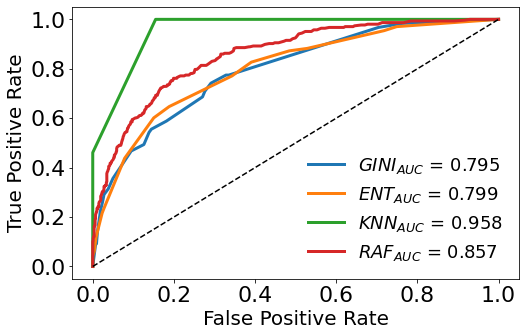
\includegraphics[width=0.8\linewidth]{semsize_ROC_c.png}\subcaption{Semantic Size}\label{fig:semroc}
\end{minipage}    \hfil
\begin{minipage}[b]{.3\linewidth}
\centering\includegraphics[width=0.8\linewidth]{masculinity_ROC_c.png}\subcaption{Masculinity}\label{fig:masroc}
\end{minipage}

\begin{minipage}[b]{.3\linewidth}
\centering\includegraphics[width=0.8\linewidth]{polysemy_ROC_c.png}\subcaption{Polysemy}\label{fig:polroc}
\end{minipage}    \hfil
\begin{minipage}[b]{.3\linewidth}
\centering\large \includegraphics[width=0.8\linewidth]{aoabinary_ROC_c.png}
\subcaption{Age of Acquisition}\label{fig:aoabinroc}
\end{minipage}    \hfil
\begin{minipage}[b]{.3\linewidth}
\centering\includegraphics[width=0.8\linewidth]{perceivability_ROC_c.png}
\subcaption{Perceivability}\label{fig:perroc}
\end{minipage}


\caption{ROC and AUC of variables}\label{fig:roc}

\end{figure}


The identification of the best model is not unique and changes from variable to variable. However, one may extract some general considerations. Regarding Decision Trees, the \textit{entropy} impurity measure generally produces a smaller error than \textit{gini}. However, one can notice that overall KNN and Random Forest perform better than Classification Trees. This behavior is confirmed by the great performance with respect to every score (accuracy, precision, recall, F1 score) as shown in Table \ref{tab:knn_scores} for the variables of interest.
One must pay attention to the fact that the good looking shape of the curves \ref{fig:arroc} and \ref{fig:semroc} for KNN is due to the low number of k, which makes it more exposed to statistical fluctuation. 

Another useful tool for the analysis of the variables of interest is given by the Confusion Matrix of Table \ref{tab:conf_matrices}. In this Matrix one can see the True Positive (TP), True Negative (TN), False Positive (FP) and False Negative (FN), as labeled in the Table.

\begin{table}[h]
    \centering
    \adjustbox{max width=\textwidth}{%
    \begin{tabular}{|r||c|c||c|c||c|c||c|}
    \hline
    & Predicted 1 & Predicted 0 & Predicted 1 & Predicted 0 & Predicted 1 & Predicted 0 &\\\hline\hline
    True 1 & \cellcolor{YellowGreen}203 &  104 & \cellcolor{YellowGreen}0 &  80 & \cellcolor{YellowGreen}279 &  159 & Decision \\\cline{1-7}\cline{1-7}
    True 0 &  41 & \cellcolor{Goldenrod}823 &  0 & \cellcolor{Goldenrod}1091 &  70 & \cellcolor{Goldenrod}663 &  Tree\\\hline\hline
    
    
    True 1 & \cellcolor{YellowGreen}207 &  100 & \cellcolor{YellowGreen}1 &  79 & \cellcolor{YellowGreen}299 &  139 & Random \bigstrut \\\cline{1-7}\cline{1-7}
    True 0 &  36 & \cellcolor{Goldenrod}828 &  2 & \cellcolor{Goldenrod}1080 &  73 & \cellcolor{Goldenrod}660 & Forest \\\hline \hline
    
    
    True 1 & \cellcolor{YellowGreen}178 &   129 & \cellcolor{YellowGreen}30 &  50 & \cellcolor{YellowGreen}276 &  162 & \multirow{2}[6]*{KNN} \bigstrut \\\cline{1-7}\cline{1-7}
    True 0 &  15 & \cellcolor{Goldenrod}849 &  13 & \cellcolor{Goldenrod}1078 &  39 &\cellcolor{Goldenrod} 694 & \\\hline \hline
    & \multicolumn{2}{|c||}{Valence} & \multicolumn{2}{|c||}{Polysemy} &
    \multicolumn{2}{|c||}{Age of Acquisition}& \\
    \hline
    \end{tabular}
    }
    \caption{Confusion Matrices for variable of interests according to the different algorithms.\\ Green indicates the True Positives, while Yellow the True Negatives.}
    \label{tab:conf_matrices}
\end{table}

This matrix highlights the fact that KNN can predict some of the few polysemyc words, unlike Decision Tree or Random Forest.  

The matrix is also helpful for the calculation of sensitivity, specificity and the other scores already mentioned. These are parameters of interest because we could give one more importance than another depending on the variable of consideration and the kind of analysis to perform. In our case, we do not have any particular need, so we look for a trade-off between precision and sensitivity. For this reason, the most useful variable for our analysis is the F1 Score, defined as a harmonic mean of the two variables mentioned above.

On one hand, one can infer that the differences between these algorithms as well as for the binary target variables are not particularly significant, because the F1 scores are not that far apart from each other. On the other hand, the differences regarding the multi-split target variables between KNN's and the algorithms' scores are more evident. 

\section{Pattern Mining}
Pattern mining is a process which allows to find out co-occurrences and patterns in our data. Firstly, we preprocessed our variables, as described in the section below. Then, we discovered the frequent itemsets and finally we extracted the association rules. 

\subsection{Preprocessing}
In order to apply a pattern discovery algorithm, we firstly normalized our dataset with the MinMaxScaler. For a better analysis, we chose to divide the range of the variables in four intervals, i.e. we  multiplied the normalized values by 3, so that each variable falls between 0 and 4. We then truncate all the variables, rounding them down. Afterwards, we added the name of the variable to its corresponding values. For the only binary variable, \textit{Polysemy}, we implemented a dictionary where 0 is \textit{not polysemic} and 1 is \textit{polysemic}. However, after some attempts in the association rules mining, we noticed that the variable \textit{polysemy} may results in just noise, without contribuiting to the analysis. That is due to the high frequency of not polysemic words in dataset, which implies an irrelevance of said variable in the rules.
Therefore, we decided to drop \textit{polysemy}.

\subsection{Frequent Itemsets}
To perform pattern extraction, we applied the \textit{apriori algorithm}, in order to find all the frequent itemsets.
%brief description of the apriori algorithm

\subsection{Choice of parameters}
The parameters to set for the \textit{apriori algorithm} are the support, the minimum number of items in a set, and the maximum items in a set. We decide to not set a limit for the max parameter. The number of frequent itemsets varying the other 2 parameters are plotted in Figure \ref{fig:itemset_parameters}. One can also look how the plots change considering only the closed and maximal itemsets. Specifically, we noticed that the green line (closed itemsets) overlaps with the yellow one (all itemsets). We then deduced that all the itemsets are closed.

\begin{figure}[h]
\begin{minipage}{0.51\linewidth}
    \centering
    \includegraphics[width=0.7\textwidth]{support.png}
    \subcaption{Number of frequent itemsets vs support (zmin=1)}
    \end{minipage}
    \hfil
    \begin{minipage}{0.46\linewidth}
    \centering
    \includegraphics[width=0.7\textwidth]{zmin.png}
    \subcaption{Number of frequent itemsets vs minimum number of elements in set (supp=6)}
    \end{minipage}
    \caption{Plots for the parameters of the apriori algorithm (frequent itemsets)}
    \label{fig:itemset_parameters}
\end{figure}

Given the dimension of the dataset, we decided to set the support parameter to 6.5\%. This choice is also due to the fact that the number of item-sets does not decrease significantly after this value.
Regarding the minimum number of elements in a set, we decided to leave the variable as loose as possible (zmin=1), because for this specific dataset it does not seem appropriate to us to exclude a priori one-to-one rules. The one-to-one rules that are not relevant will be left out by the confidence or lift threshold. 

\begin{minipage}{0.48\linewidth}

\begin{table}[H]
    \centering
        \adjustbox{max width=0.9\textwidth}{%
        \begin{tabular}{|r||c|c|c|c|c|}
    \toprule
         Confidence &  0.50 & 0.60 & 0.70 & 0.80 & 0.90  \\
         \hline
         Number of rules & 743 & 216 & 62 & 26 & 3 \\\midrule \midrule
         Lift & 1.5 & 1.6 & 1.7 & 1.8 & 2.2 \\\hline
         Number of rules & 33 & 22 & 11 & 9 & 2\\
         \bottomrule
    \end{tabular}
    }
   
        \caption{Number of rules by confidence and lift} \label{tab:par_rules}

\end{table}
\end{minipage}
\hfil
\begin{minipage}{0.48\linewidth}
\centering
\begin{table}[H]
    \centering
        \adjustbox{max width=0.9\textwidth}{%

    \begin{tabular}{|c|c|c|}
    \toprule
    Word & Target Variable & Counts \\\midrule\midrule
         Christmas & 7.0 Web Corpus Freq & 2\\\hline
         Dad & 7.0 Web Corpus Freq & 6 \\\hline
         FALSE & 6.0 Web Corpus Freq & 3\\  \hline
         FALSE & 7.0 Web Corpus Freq & 1 \\\hline
         Mom & 7.0 Web Corpus Freq & 7 \\\hline
         Mum & 7.0 Web Corpus Freq & 3 \\\hline
         Mummy & 7.0 Web Corpus Freq & 2 \\\hline
         TRUE & 7.0 Web Corpus Freq & 1\\\hline
         TV & 7.0 Web Corpus Freq & 10 \\\hline
         Twitter & 7.0 Web Corpus Freq & 1\\\hline
         yo-yo & 6.0 Web Corpus Freq & 6\\
         \bottomrule
    \end{tabular}
    }
            \caption{Prediction and counts for missing values} \label{tab:miss_ass}

\end{table}

\end{minipage}

\subsection{Association Rules extraction}
The Association Rules are extracted using the \textit{apriori algorithm}.
Varying the parameters of confidence and lift we obtained different number of rules. First, we vary the confidence parameter in a range between 0.50 and 0.90. Once decided to put the threshold at 75\% for the confidence we varied the lift in a range from 1.5 to 2.2. The results are shown in Table \ref{tab:par_rules}.


The threshold for the lift is set at 1.6. The obtained rules, ordered by target and lift, are reported in Table \ref{tab:rules}.

\begin{table}[h]
    \centering
\adjustbox{max width=0.85\textwidth}{%
\begin{tabular}{|r|l|c|r|r|r|r|}
\toprule
{} &                                         Antecedent &              Target &  Lift &  Conf &  Supp (\%) &  Supp \\
\midrule\midrule
1  &                                     (0.0\_SemSize,) &  3.0\_Perceivability &  2.45 &  0.76 &      7.78 &   363 \\\hline
2  &      (0.0\_Age\_of\_Acquisition, 7.0\_Web\_Corpus\_Freq) &     3.0\_Familiarity &  2.23 &  0.93 &      7.26 &   339 \\\hline
3  &            (0.0\_Age\_of\_Acquisition, 2.0\_Dominance) &     3.0\_Familiarity &  2.16 &  0.90 &      8.53 &   398 \\\hline
4  &          (0.0\_Age\_of\_Acquisition, 1.0\_Masculinity) &     3.0\_Familiarity &  2.16 &  0.90 &      7.46 &   348 \\\hline
5  &               (0.0\_Age\_of\_Acquisition, 0.0\_Lenght) &     3.0\_Familiarity &  2.11 &  0.88 &     10.00 &   467 \\\hline
6  &                          (0.0\_Age\_of\_Acquisition,) &     3.0\_Familiarity &  2.08 &  0.87 &     14.29 &   667 \\\hline
7  &              (0.0\_Age\_of\_Acquisition, 2.0\_Valence) &     3.0\_Familiarity &  2.07 &  0.87 &      8.78 &   410 \\\hline
8  &       (0.0\_Age\_of\_Acquisition, 3.0\_Perceivability) &     3.0\_Familiarity &  2.05 &  0.86 &      8.27 &   386 \\\hline
9  &              (0.0\_Age\_of\_Acquisition, 1.0\_Arousal) &     3.0\_Familiarity &  2.03 &  0.85 &      6.79 &   317 \\\hline 
10 &   (3.0\_Perceivability, 2.0\_Dominance, 1.0\_Arousal) &         2.0\_Valence &  1.77 &  0.90 &      8.05 &   376 \\\hline
11 &  (7.0\_Web\_Corpus\_Freq, 2.0\_Dominance, 1.0\_Arousal) &         2.0\_Valence &  1.74 &  0.88 &      6.75 &   315 \\\hline
12 &  (3.0\_Perceivability, 3.0\_Familiarity, 1.0\_Arou... &         2.0\_Valence &  1.68 &  0.85 &      6.51 &   304 \\\hline
13 &      (3.0\_Familiarity, 2.0\_Dominance, 1.0\_Arousal) &         2.0\_Valence &  1.68 &  0.85 &      8.63 &   403 \\\hline
14 &          (1.0\_SemSize, 2.0\_Dominance, 1.0\_Arousal) &         2.0\_Valence &  1.67 &  0.84 &      8.40 &   392 \\\hline
15 &              (3.0\_Perceivability, 1.0\_Masculinity) &         2.0\_Valence &  1.64 &  0.83 &      8.61 &   402 \\\hline
16 &      (1.0\_Masculinity, 2.0\_Dominance, 1.0\_Arousal) &         2.0\_Valence &  1.64 &  0.83 &      6.62 &   309 \\\hline
17 &      (2.0\_Dominance, 1.0\_Arousal, 2.0\_Masculinity) &         2.0\_Valence &  1.63 &  0.82 &      9.06 &   423 \\\hline
18 &  (3.0\_Perceivability, 3.0\_Familiarity, 2.0\_Domi... &         2.0\_Valence &  1.62 &  0.82 &      8.20 &   383 \\\hline
19 &           (2.0\_Dominance, 1.0\_Arousal, 1.0\_Lenght) &         2.0\_Valence &  1.61 &  0.82 &      8.80 &   411 \\\hline
20 &      (1.0\_SemSize, 3.0\_Familiarity, 2.0\_Dominance) &         2.0\_Valence &  1.61 &  0.81 &      6.79 &   317 \\\hline
21 &    (3.0\_Perceivability, 2.0\_Dominance, 1.0\_Lenght) &         2.0\_Valence &  1.60 &  0.81 &      6.68 &   312 \\\hline
22 &                         (3.0\_Valence, 2.0\_SemSize) &       2.0\_Dominance &  1.69 &  0.76 &      6.90 &   322 \\
\bottomrule
\end{tabular}
}
        \caption{Association Rules with a confidence$\geq75\%$, lift$\geq1.6$ and support$\geq6.5\%$}\label{tab:rules}

\end{table}

\subsection{Replacing Missing Values}
A useful aspect of the Association Rules is the replacement of missing values with some more accurate predictions. However, in our case the only variable that has missing value is \textit{Web Corpus Frequency} (Figure \ref{fig:missing}), which does not appear as a target variable for our rules. One could look for new rules with this target variable lowering the support, the confidence and the lift. In order to do so, we set the parameters respectively to 2, 50 and 1.3. To decrease the noise, we set a threshold at zmin=2. We then counted how many rules would predict a specific value for the a word without a \textit{Web Corpus Frequency} value. The obtained results are shown in Table \ref{tab:miss_ass}.


For the results with a high count (e.g. TV, Mom, yo-yo) one may replace the predicted value for \textit{Web Corpus Frequency}. However, the lift, support and confidence for the majority of these rules are not quite good.

Trying to tighten up the cuts on the parameters (supp>4, conf>60, lift>1.4), one find only one rule that predict the missing value for the words in Table \ref{tab:miss_ass}. This rule applies only for yo-yo and predicts the same result shown in the table.


\subsection{Final Discussion}

In the choice of the threshold for the confidence and the lift we opted for a balance between quantity and quality of the rules. 

The obtained rules in Table \ref{tab:rules} all have a high lift and the majority has as target the variable \textit{Valence}. However, the variable \textit{Familiarity} is the one with the most interesting rules, because of its high lift and confidence. We can also notice the negative correlation between \textit{age of acquisition} and \textit{Familiarity}: every high value for \textit{Familiarity} is predicted by a low value of \textit{Age of Acquisition}.

Regarding the replacement of missing values, one can only infer quite certainly that the word \textit{yo-yo} has a \textit{Web Corpus Frequency} value of 6. Given the fact that the words in Table \ref{tab:miss_ass} seem common, the results for the other words appear reasonable. However, these predictions have a low confidence and lift level, so there is no certainty of their accuracy.
%commento sul fatto che regole trovate sono buone e hanno lift alto e che se ne potrebbero avere anche di più variando di poco i parametri (support, confidence, lift). Abbiamo scelto di tenere poche regole (quindi fare tagli alti) per verificarle coi tree delle target variable. 
%confronto con tree (familiarity, valence, dominance?)
%inseriamo immagine del tree di valence (L'HO GIA' MESSA NELLA PARTE DI PRUNING) e facciamo vedere due esempi di regole che performano bene.

%Se riusciamo a trovare un modo migliore per comparare association rules e decision tree meglio (...)


\section{Conclusions}

The Glasgow Norms has resulted to be an interesting dataset to work with.

The application of unsupervised and supervised algorithms has shown some trends. For instance, there is a group of words, belonging to the sixth cluster (from the Hierarchical Clustering algorithm) which are short in length, acquired in early age and very familiar: this is reflected in the fifth association rule \textit{((0.0 Age of Acquisition, 0.0 Length)} $\Rightarrow$ \textit{3.0 Familiarity)}
in Table \ref{tab:rules}. Similarly, the third cluster (from the Hierarchical Clustering algorithm) contains words with high valence, high dominance and high semantic size: an extracted rule (n. 22 in Table \ref{tab:rules}) implies that words with high valence and semantic size are high in dominance as well. 

\textit{Valence} proves to be a good target variable for classification, with high accuracy, precision, recall and F1-score; at the same time, it is a consequent (meaning target variable) for a large number of extracted rules. 

The same is true for the variable \textit{Familiarity}, which proves to be an interesting variable also because of its high anti-correlation with \textit{Age of Acquisition}. One can compare the rules found with the classification tree obtained in Section \ref{target_dt} and shown in Figure \ref{fig:tree_fam}. The variables used to split the tree confirm the found association rules completely.
\begin{figure}[h]
    \centering
    \includegraphics[width=0.9\textwidth]{fam_tree_entropy.png}
    \caption{Familiarity Decision Tree}
    \label{fig:tree_fam}
\end{figure}
On the other hand, the only binary parameter, \textit{Polysemy}, was not a satisfying target variable, given the imbalance of its distribution: the large majority of words in the dataset are not polysemic. Thus, leading to inaccurate or unexpected results during the clustering, %controllare 
classification and pattern mining tasks.



%considerazioni generali
\newpage
%\pagenumbering{roman} % Start roman numbering
\nocite{*}
\printbibliography

\end{document}

